\documentclass[]{article}
\usepackage{caption,subcaption,graphicx,float,url,amsmath,amssymb,tocloft,cancel}
\usepackage[hidelinks]{hyperref}
\usepackage[toc,acronym,nonumberlist]{glossaries}
\usepackage{titling}
\setacronymstyle{long-short}
\usepackage{glossaries-extra}
\graphicspath{{figs/}} 
\setlength{\cftsubsecindent}{0em}
\setlength{\cftsecnumwidth}{3em}
\setlength{\cftsubsecnumwidth}{3em}
\pretitle{
	\begin{center}
		
\includegraphics[width=6cm]{KanjiLife}\\
		
	}
	\posttitle{\end{center}}

%opening
\title{
	Notes from Origins of Life\\
	Week 5: Evolution}
\author{Simon Crase (compiler)\\simon@greenweaves.nz}

\makeglossaries

\loadglsentries{glossary-entries}

\renewcommand{\thesection}{5.\arabic{section}}
\renewcommand{\glstextformat}[1]{\textbf{\em #1}}
\newcommand{\E}{\mathrm{E}}
\newcommand{\Var}{\mathrm{Var}}
\newcommand{\Cov}{\mathrm{Cov}} 
\newcommand\numberthis{\addtocounter{equation}{1}\tag{\theequation}}

\begin{document}

\maketitle

\begin{abstract}
   These are my notes from the $5^{th}$ Week of the Santa Fe Institute Origins of Life Course\cite{sfi2020}. 
   The content and images contained herein are the intellectual property of the Santa Fe Institute, with the exception of any errors in transcription, which are my own.
   These notes are distributed in the hope that they will be useful,
   but without any warranty, and without even the implied warranty of
   merchantability or fitness for a particular purpose. All feedback is welcome,
   but I don't necessarily undertake to do anything with it.
\end{abstract}

\setcounter{tocdepth}{2}
\tableofcontents
\listoffigures

\section[Introduction]{Introduction--Chris Kempes}

We discuss Selection, \gls{gls:phylogenetics}, Macroscopic Regularities across all of life, how  life has evolved in creating Complexity, and evolutionary processes in Artificial Life. 

\section[Origins of Eukaryotes]{Origins of Eukaryotes--David Baum}

\subsection{Prokaryotes and Eukaryotes}

Since life originated, perhaps 4 billion years ago, on this planet, most people would say that the most important subsequent transition was the evolutionary origin of the eukaryotes--the origin of large, complex cells such as we find in the bodies of animals, plants, and fungi. The origin lf eukaryotes is a distinct problem to the origin of life, but it shares the features that we don't have intermediate steps, and it happened just once. It can serve as a model for studying difficult and rare transitions.

Cellular life began \gls{gls:prokaryotic}-- \glsdesc{gls:prokaryotic}
boundary--Figure \ref{fig:prokaryote}. Structurally \gls{gls:prokaryotic} cells are very simple, but we must remember that the \gls{gls:cytoplasm} is very complicated at the biochemical and genetic level.

\begin{figure}[H]
	\begin{center}
		\caption{Cellular life began \gls{gls:prokaryotic}}\label{fig:prokaryote}
		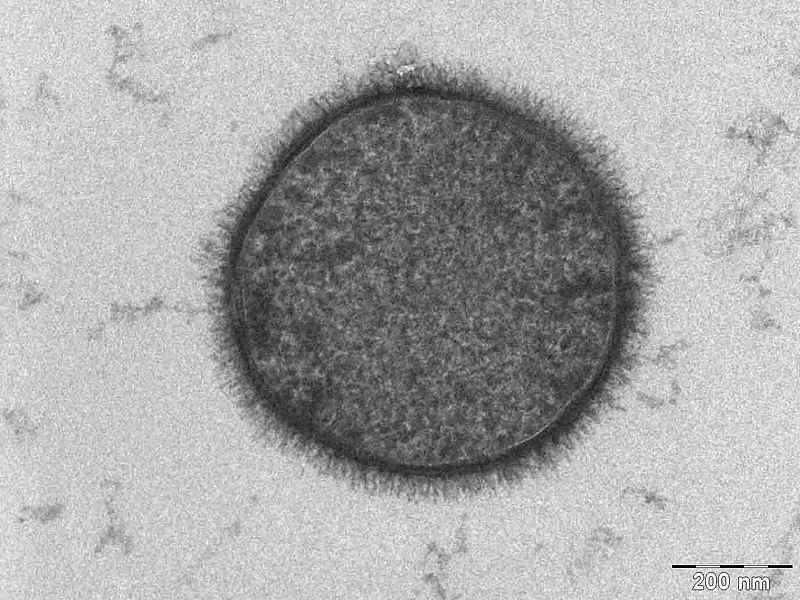
\includegraphics[width=0.6\textwidth]{prokaryote}
	\end{center}
\end{figure}

\Gls{gls:eukaryotic} cells are structurally complex--Figure \ref{fig:ManyMembranes}. 

\begin{itemize}
	\item They are larger
	\item They have multiple internal membrane-bound structures
	\begin{itemize}
		\item \emph{nucleus} enclosed genetic material
		\item \emph{mitochondria} generate energy for the cell
		\item endomembrane system
	\end{itemize}
	\item We know they arose just once.
\end{itemize}

\begin{figure}[H]
	\caption[\Gls{gls:eukaryotic} cells: multiple internal membrane-bound structures]{\Gls{gls:eukaryotic} cells have multiple internal membrane-bound structures}\label{fig:ManyMembranes}
	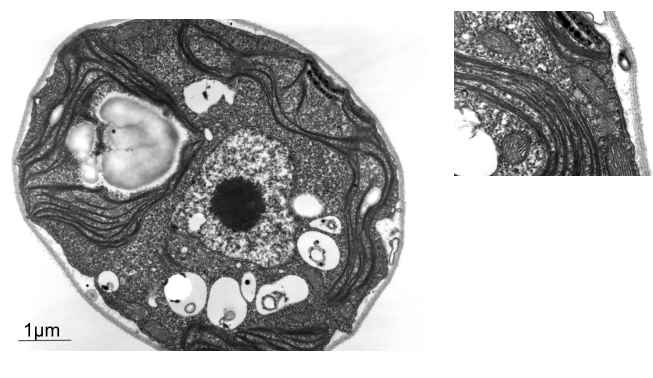
\includegraphics[width=0.8\textwidth]{ManyMembranes}
\end{figure}

So \gls{gls:eukaryotic} cells are significantly different from \gls{gls:prokaryotic} cells, and we have no intermediates known between these two states of being.

\begin{itemize}
	\item Eukaryotes are cellular predators--Figure \ref{figs:Cellular:predators:symbiotic:hosts1}--the lions and tigers of the micro-biotic world!
	\item Eukaryotes are symbiotic hosts--Figure \ref{figs:Cellular:predators:symbiotic:hosts2}-- the farmers of the micro-biotic world! They can take in other cells, mostly prokaryotes, shelter them, and foster a close intimate relationship. The best known example is photosynthesis: algae and plants enclose formerly free-living photosynthetic bacteria as chloroplasts.
\end{itemize}

\begin{figure}[H]
	\caption{Cellular predators, symbiotic hosts}
	\label{figs:Cellular:predators:symbiotic:hosts}
	\begin{subfigure}[b]{0.45\textwidth}
		\caption{ Cellular predators}
		\label{figs:Cellular:predators:symbiotic:hosts1}
		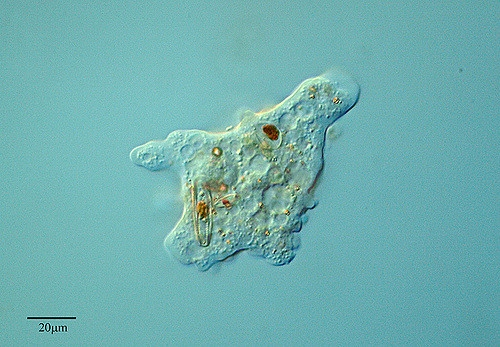
\includegraphics[width=\textwidth]{Eukaryotes1}
	\end{subfigure}
	\begin{subfigure}[b]{0.45\textwidth}
		\caption{Symbiotic hosts }
		\label{figs:Cellular:predators:symbiotic:hosts2}
		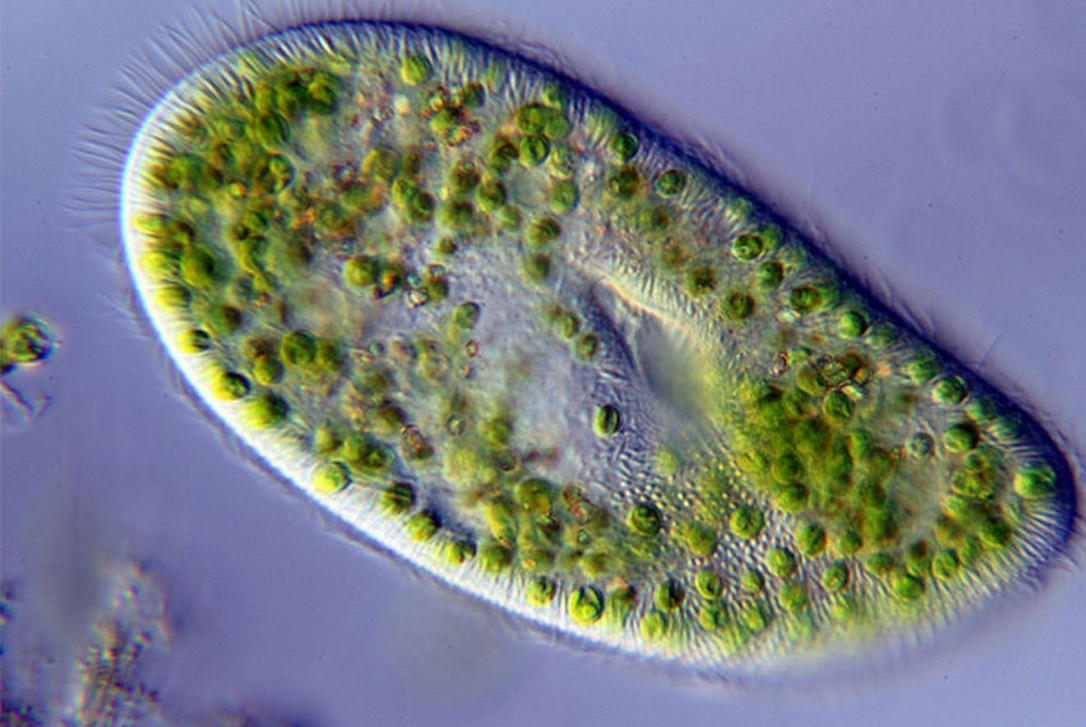
\includegraphics[width=\textwidth]{Eukaryotes2}
	\end{subfigure}
\end{figure}

The other thing that only eukaryotes do is the formation of multicellular organisms--Figure \ref{fig:multicellularity}. This is a sophisticated form of multicellularity, where cells have specialized, and only one kind of cell is able to pass on its genes to the next generation.

\begin{itemize}
	\item why have only eukaryotes evolved multicellularity?
	\item why have eukaryotes evolved multicellularity multiple times? (The best known instances are animals, plants, and fungi, but there are others.)
\end{itemize}

\begin{figure}[H]
	\caption{A significant evolutionary event--Multicellularity}\label{fig:multicellularity}
	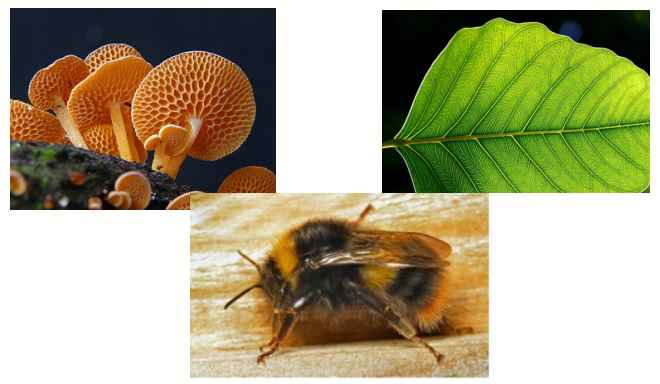
\includegraphics[width=0.8\textwidth]{multicellularity}
\end{figure}

\subsection{Why eukaryotes?}
Why eukaryotes? There are three ideas at present.

\begin{itemize}
	\item Mitochondria improve energetic efficiency, and allow energy use to be regulated more nimbly--Figure \ref{fig:EukaryotesMoreEfficient}.
	
	\item Flexible membranes allow phagocytosis and generation of internal vesicles. So eukaryotes can do things that prokaryotes can't, such as engulfing food prey--Figure \ref{fig:engulf}.
	
	\item Nucleus and \gls{gls:endomembrane} system allow for many more levels of gene
	regulation--Figure \ref{fig:finer:gene:regulation}--and this may be a reason why eukaryotes alone have evolved multi-cellularity.
	\begin{itemize}
		\item Multicellular organization requires communications between different cells, which express different genes and proteins.
		\item The extra layers of regulation that eukaryotes have may explain why they, and not prokaryotes, have evolved complex multicellular organisms. 
		\begin{itemize}
			\item These layers deal with the genetic control by separating the transcription of a \gls{gls:DNA} sequence from the reading of the message--there are many steps where regulation can be imposed. 
			\item Additionally the \gls{gls:endomembrane} system can affect the secretion, degradation and recycling of proteins
		\end{itemize}
	\end{itemize}
\end{itemize}

\begin{figure}[H]
	\begin{center}
		\caption[Mitochondria improve energetic efficiency]{Mitochondria improve energetic efficiency, and allow energy use to be regulated more nimbly\cite{lane2010energetics}}\label{fig:EukaryotesMoreEfficient}
		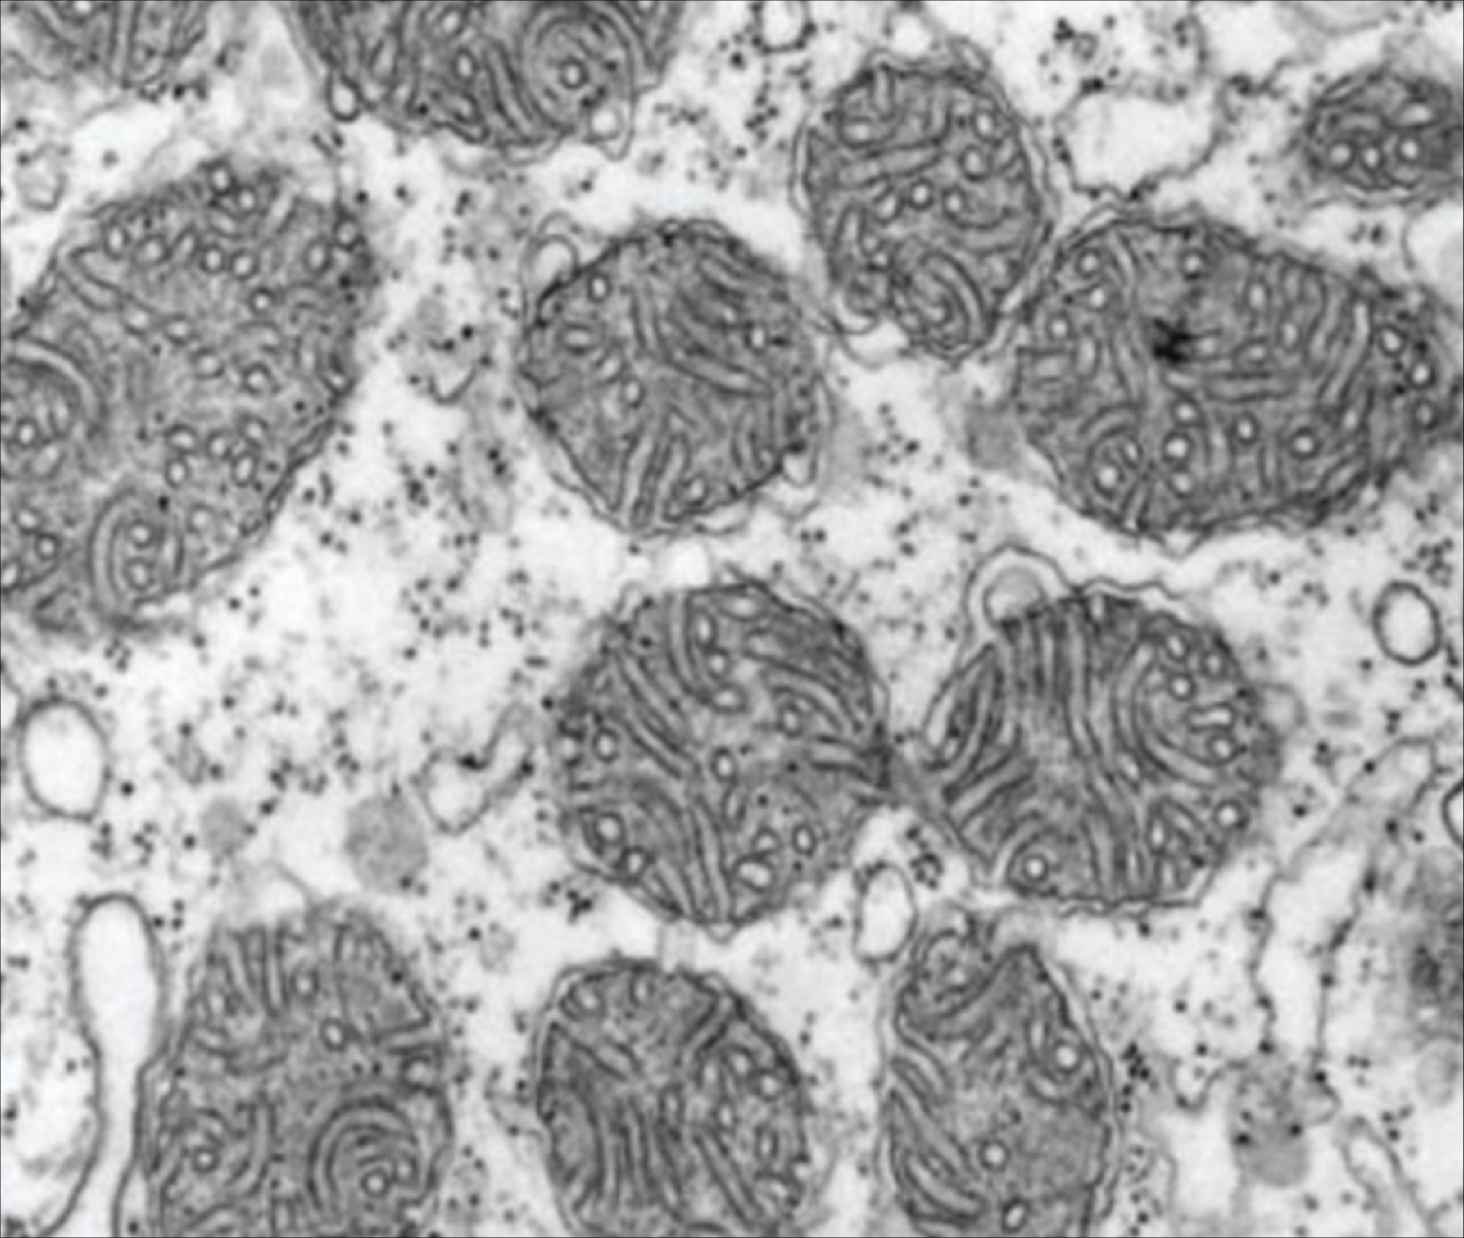
\includegraphics[width=0.6\textwidth]{EukaryotesMoreEfficient}
	\end{center}
\end{figure}

\begin{figure}[H]
	\caption[Flexible membranes]{Flexible membranes allow phagocytosis and generation
		of internal vesicles}
	\label{fig:engulf}
	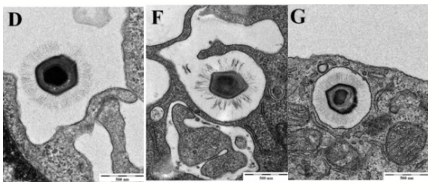
\includegraphics[width=0.9\textwidth]{Engulf}
\end{figure}

\begin{figure}[H]
	\caption[Nucleus and endomembrane system allow for finer gene
		regulation]{Nucleus and endomembrane system allow for finer gene
		regulation\cite{paez2016endocytosis}}\label{fig:finer:gene:regulation}
	\begin{subfigure}[b]{0.45\textwidth}
		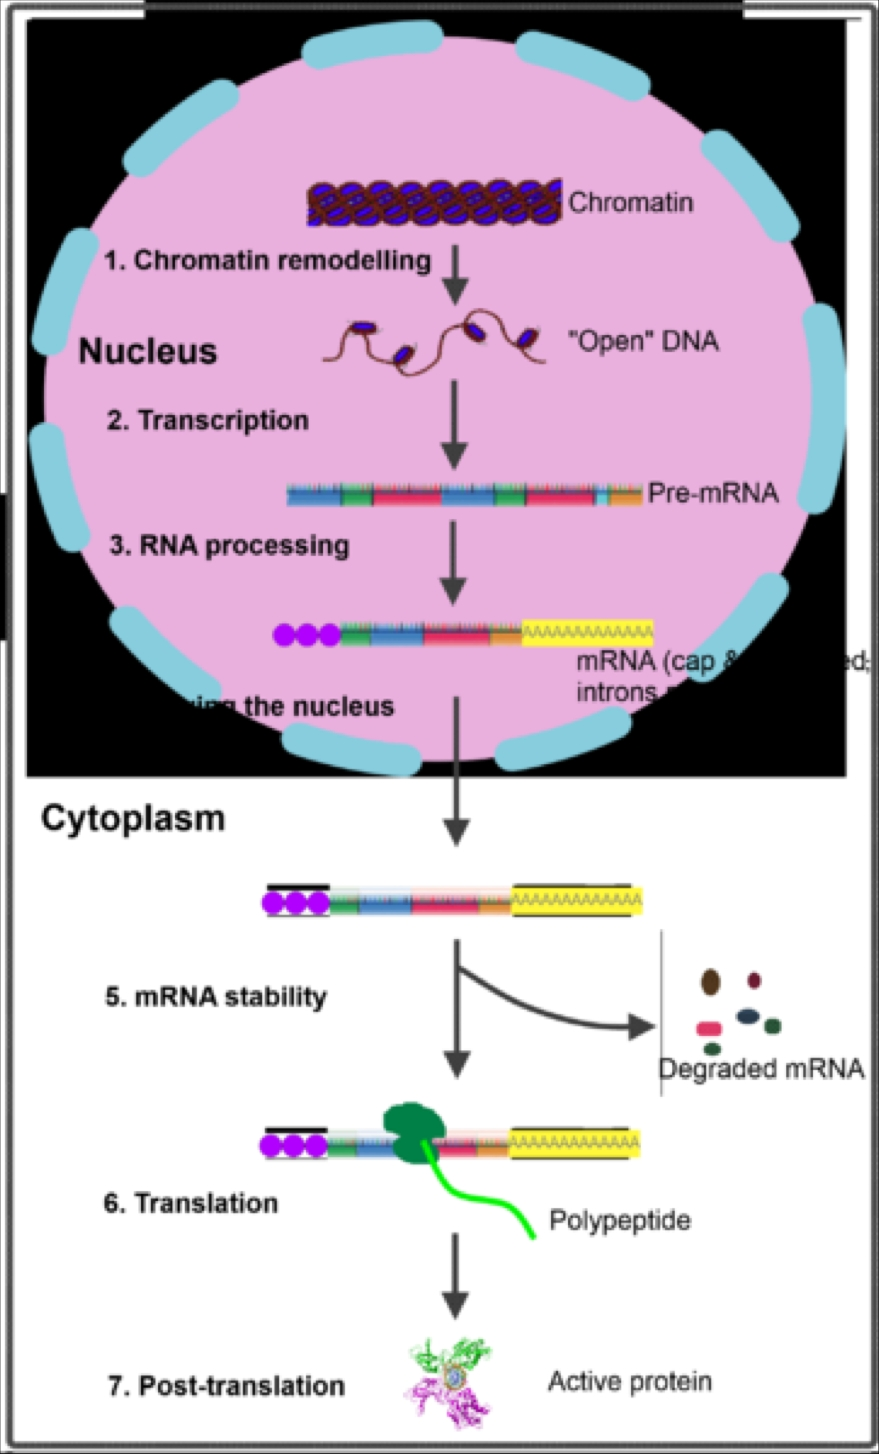
\includegraphics[width=\textwidth]{Regulation1}
	\end{subfigure}
	\begin{subfigure}[b]{0.45\textwidth}
	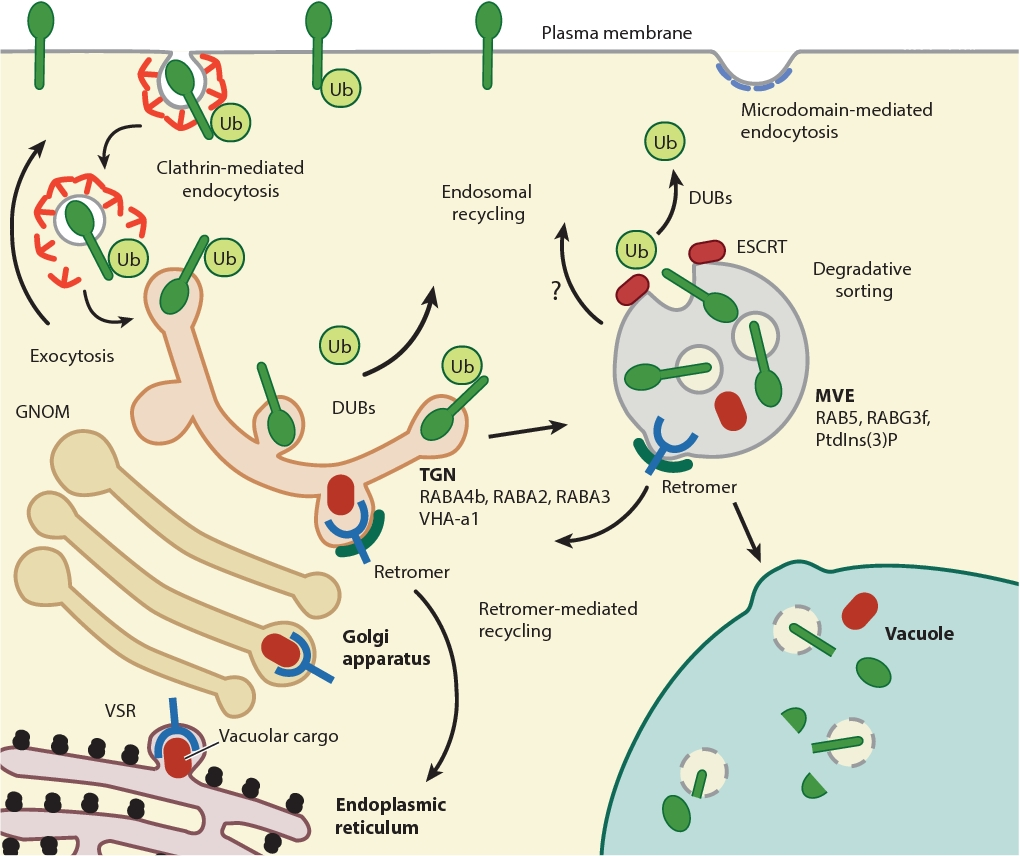
\includegraphics[width=\textwidth]{Regulation2}
	\end{subfigure}
\end{figure}

These are some of the reasons why we believe that the eukaryotic transition is well worth studying. Like the origin of life, this is a unique event, but we do have one great advantage in this area:  we can use phylogenetic methods to study both ends of the stem lineage of the eukaryotes.


\begin{itemize}
	\item We can use phylogenetic inference  to reconstruct the trace of \gls{gls:LECA}--Figure \ref {fig:LECA}.
	
	\item We can also go down to the end of that stem lineage and identify and infer traits of ancestors of \gls{gls:LECA}.
	
	\item  We cannot do this with \gls{gls:LUCA}, as we hit a phylogenetic singularity.

\end{itemize}

\begin{figure}[H]
	\caption[We can use phylogenetic inference  to reconstruct the trace of LECA]{We can use phylogenetic inference  to reconstruct the trace of \gls{gls:LECA}}\label{fig:LECA}
	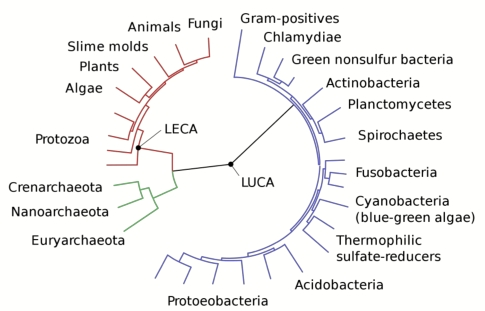
\includegraphics[width=0.9\textwidth]{LECA}
\end{figure}

We can use phylogenetic methods, and there are things that we have been able to figure out about the origin of the eukaryotes that are quite significant:
\begin{itemize}
	\item Mitochondria are endosymbiotic bacteria, descended from alphaproteobacteria--Figure \ref{fig:Mitochondria:are:endosymbiotic:bacteria}. These bacteria were taken up by the ancestral eukaryote and integrated into the cell, but did not completely lose their genome.
	\item Host was an archaeon--Figure \ref{fig:host:archaeon}
	\item We can distinguish genes of archaeal or 	bacterial ancestry--Figure \ref{fig:distinguish:genes:archaeal:bacterial}--in modern eukaryotes. This is helpful for figuring out how disparate cells came together for firm a coherent organism.
\end{itemize}

\begin{figure}[H]
	\begin{center}
		\caption[Mitochondria are endosymbiotic bacteria]{Mitochondria are endosymbiotic bacteria\cite{germot1996presence}} 	\label{fig:Mitochondria:are:endosymbiotic:bacteria}
		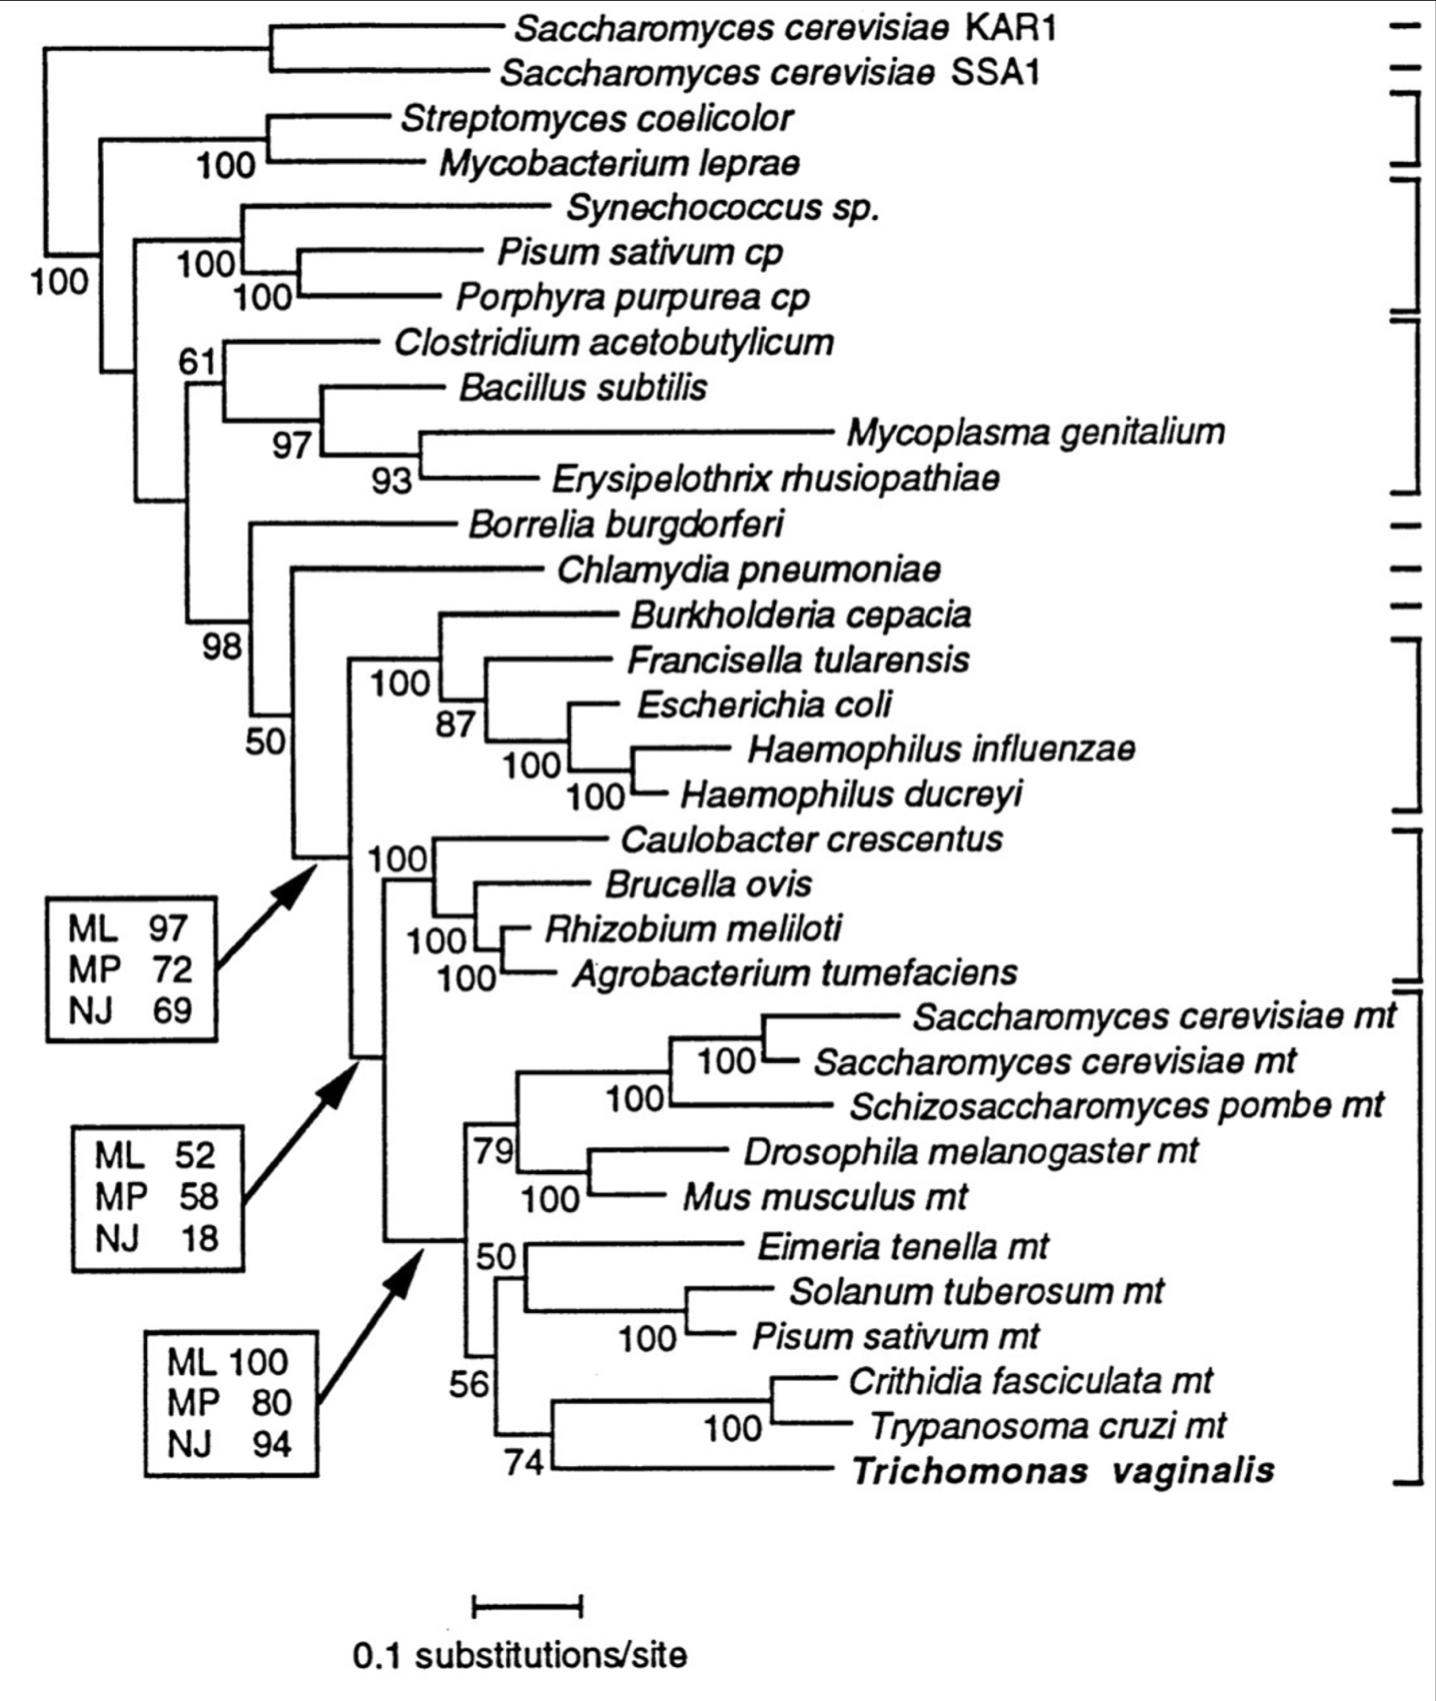
\includegraphics[width=0.9\textwidth]{MitochondriaEndosymbiotic}
	\end{center}
\end{figure}

\begin{figure}[H]
	\caption[Host was an archaeon]{Host was an archaeon\cite{spang2015complex}}
	\label{fig:host:archaeon}
	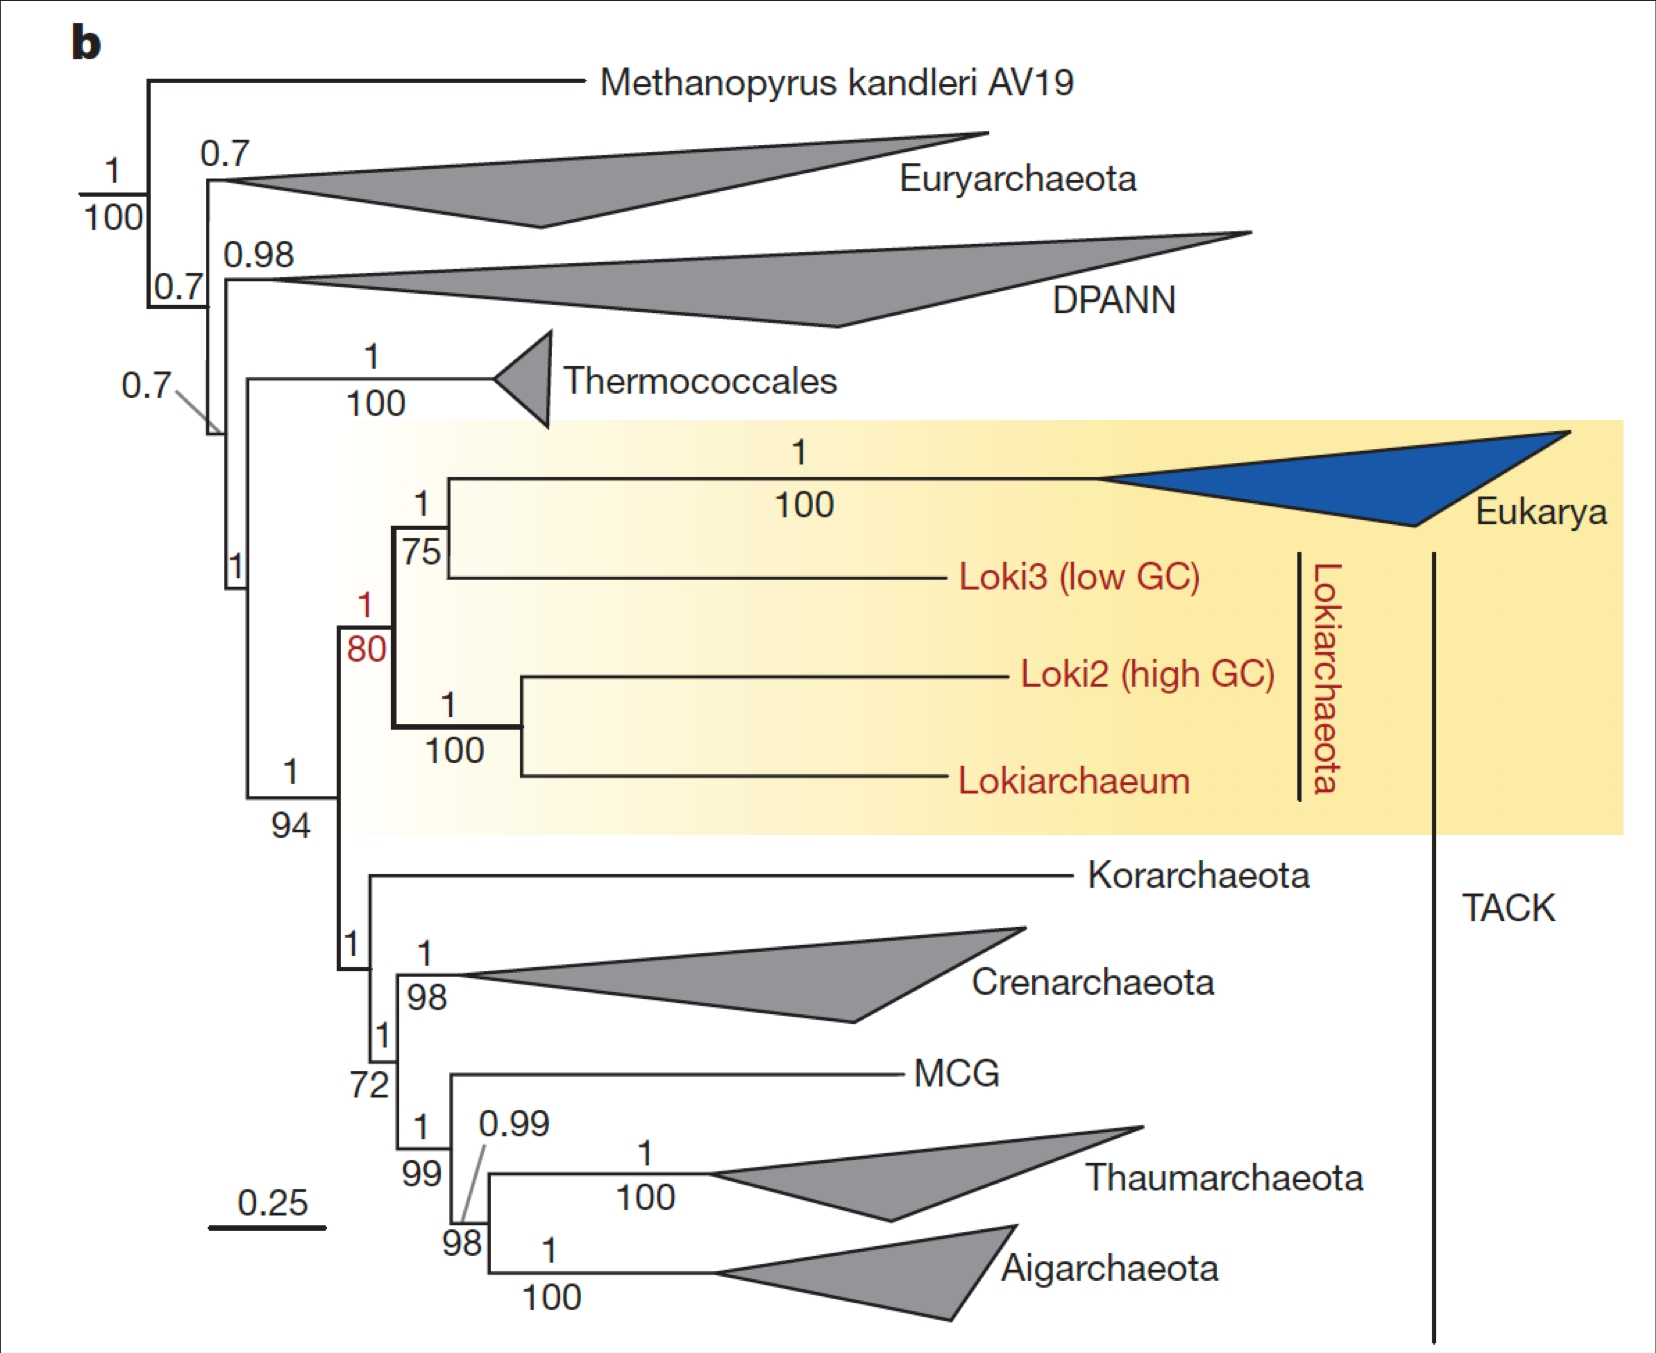
\includegraphics[width=0.9\textwidth]{HostArchaeon}
\end{figure}

\begin{figure}[H]
	\caption[Can distinguish genes of archaeal or bacterial ancestry]{Can distinguish genes of archaeal or bacterial ancestry\cite{thiergart2012evolutionary}}
	\label{fig:distinguish:genes:archaeal:bacterial}
	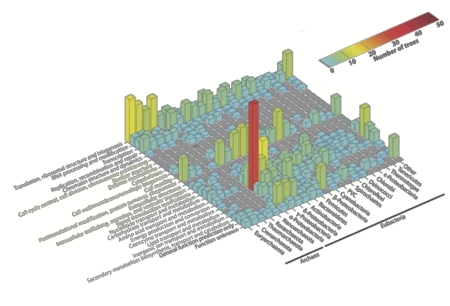
\includegraphics[width=0.9\textwidth]{thiergart2012}
\end{figure}

Mysteries remain. They are generally structural problems. We can reconstruct the history of genes from their sequences. Membranes and structures don't have genes, so we can't infer their history. Instead we have to come up with scenarios and plausibility arguments to answer questions such as the following. 

\begin{itemize}
	\item How did a bacterium get into an archaeon? 
	\item How was a nucleus formed?
\end{itemize}

There are two extremes in a range of theories.
\begin{itemize}
	\item In the Outside-in Model, an ancestral archaeon had a membrane, Figure \ref{fig:outside:in1}, which became invaginated. It enveloped a bacterium in a mutualistic association--Figure \ref{fig:outside:in2}. Later it assembled membranes and vesicles to build a compartment to protect \gls{gls:DNA} from the activity (free oxygen) of the mitochondria--Figure \ref{fig:outside:in3}--until the nucleus was stabilized with the addition of the nuclear pores--Figure \ref{fig:outside:in4}.
	\item In the Inside-out Model--Figure \ref{fig:inside:out}--the archaeon host becomes associated with extra-cellular bacteria, which are gradually walled in.
\end{itemize}

\begin{figure}[H]
	\caption{Origin of membranes and structures: Outside-in Model}\label{fig:outside:in}
	\begin{subfigure}[b]{0.45\textwidth}
		\caption{Ancestral archaeon had a membrane which became invaginated }\label{fig:outside:in1}
		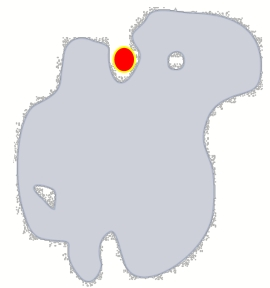
\includegraphics[width=\textwidth]{OutsideIn1}
	\end{subfigure}
	\begin{subfigure}[b]{0.45\textwidth}
		\caption{ Cell gradually enveloped mitochondria in a mutualistic association. It enveloped a bacterium in a mutualistic association.}\label{fig:outside:in2}
		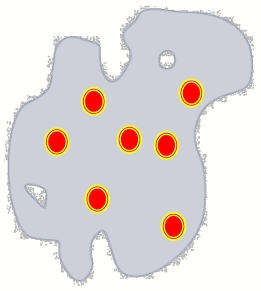
\includegraphics[width=\textwidth]{OutsideIn2}
	\end{subfigure}
	\begin{subfigure}[b]{0.45\textwidth}
		\caption{Cell later assembled membranes and vesicles to build a compartment to protect \gls{gls:DNA} from the activity (free oxygen) of the mitochondria}\label{fig:outside:in3}
		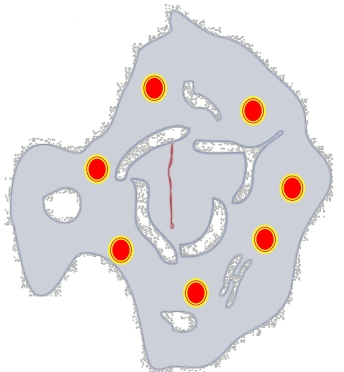
\includegraphics[width=\textwidth]{OutsideIn3}
	\end{subfigure}
	\begin{subfigure}[b]{0.45\textwidth}
		\caption{Eventually the nucleus was stabilized with the addition of the nuclear pores}\label{fig:outside:in4}
		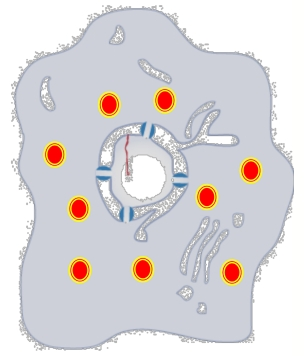
\includegraphics[width=\textwidth]{OutsideIn4}
	\end{subfigure}
\end{figure}

\begin{figure}[H]
	\caption[Origin of membranes and structures: Inside-Out Model]{Origin of membranes and structures: Inside-Out Model\cite{baum2014inside}. A mutualistic relationship is established, and the host extrudes membranes structures, ''blebs'', that gradually formed an external structure to trap and enclose the mitochindria. Finally the structure fused to form a new compartment that enclosed the cytoplasm. The original archaeon became the nucleus.}\label{fig:inside:out}
	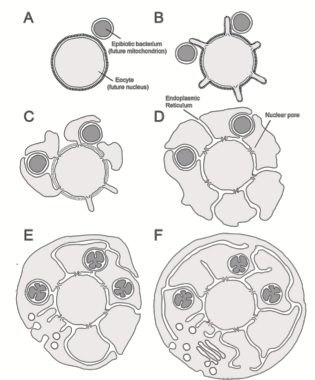
\includegraphics[width=0.9\textwidth]{InsideOut}
\end{figure}

At present we cannot distinguish between these two stories, but there is a hope that new genomic data will enable us to do this.

\begin{itemize}
	\item New genomic data keep emerging
	\item There is a possibility of finding intermediates
\end{itemize}

\begin{figure}[H]
	\begin{center}
		\caption[Prospects for distinguishing between the two stories]{Prospects for distinguishing between the two stories\cite{javaux2003recognizing}}\label{fig:Javaux}
		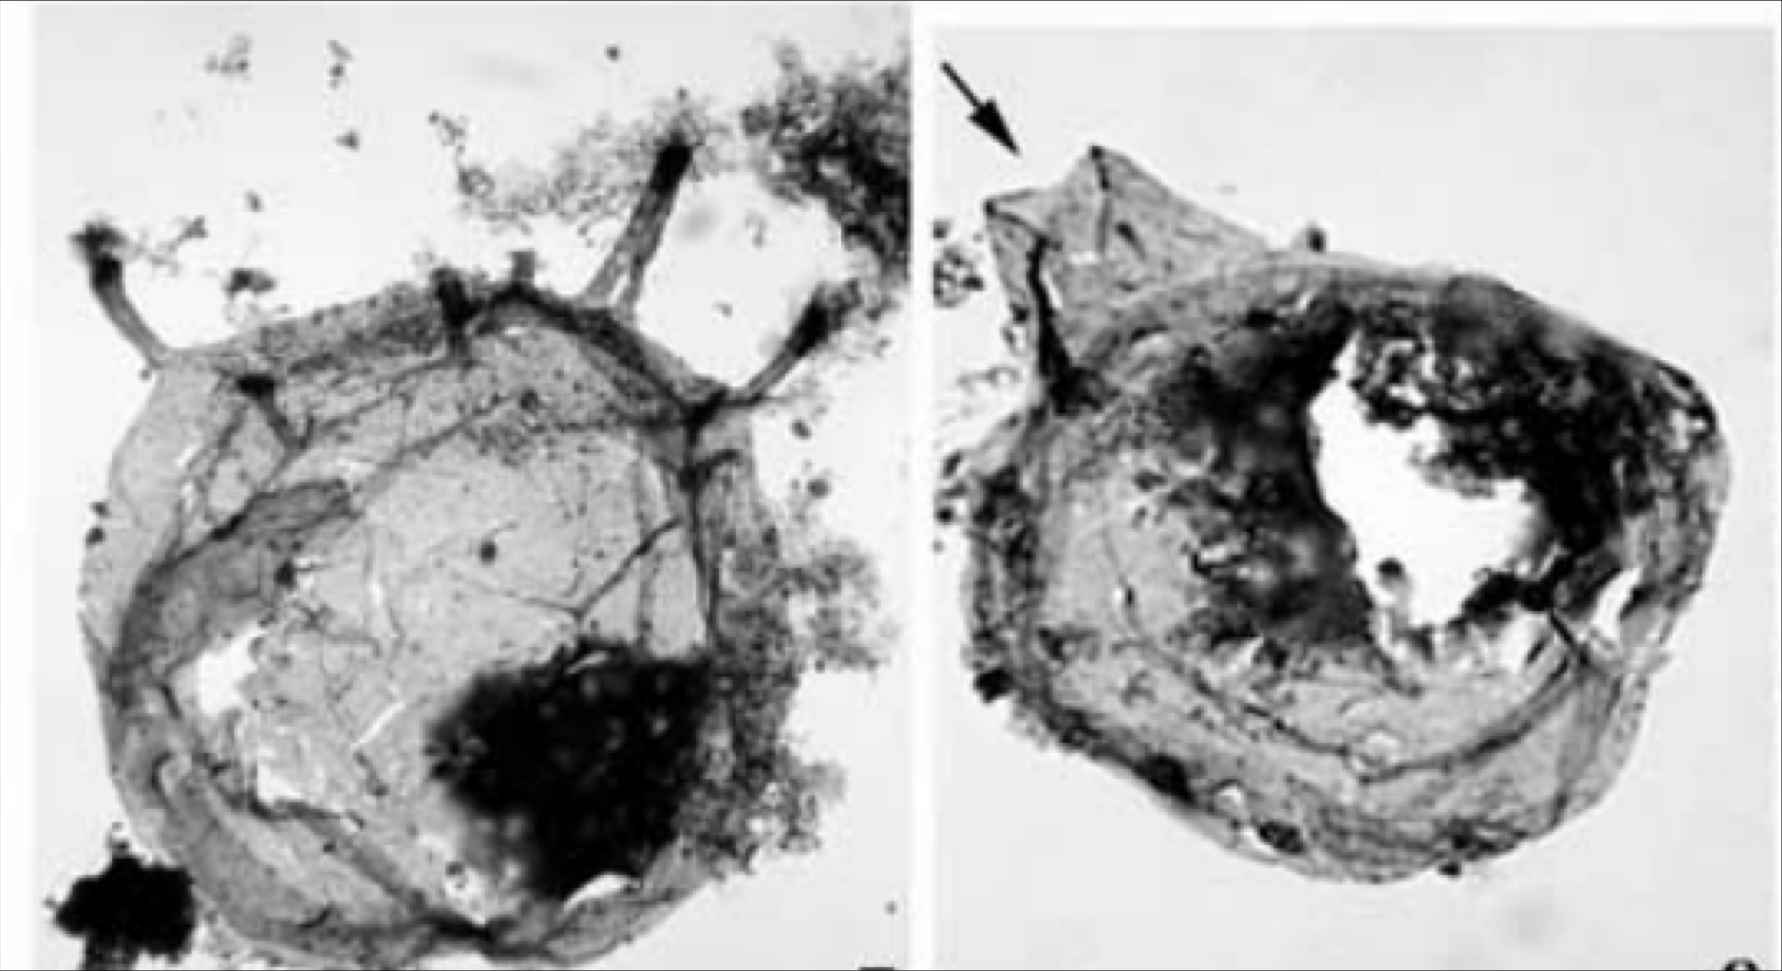
\includegraphics[width=0.6\textwidth]{Javaux}
	\end{center}
\end{figure}
  

\section{Phylogenetics}


\subsection[Using Phylogenetics to Travel in Time]{Using Phylogenetics to Travel in Time--Bet{\"u}l Ka{\c c}ar}

Today we will be talking about \gls{gls:phylogenetics} and how to make sense of phylogenetic trees.
\subsubsection{what is a phylogenetic tree?}

Consider these very different organisms: a flower, bacteria, an elephant, a giraffe, an orange, a human being--Figure \ref{fig:WhatDoTheseSpeciesHaveInCommon}.
As different as they are, what do all these species have in common?
\begin{figure}[H]
	\begin{center}
		\caption{What do these Species have in Common?}\label{fig:WhatDoTheseSpeciesHaveInCommon}
		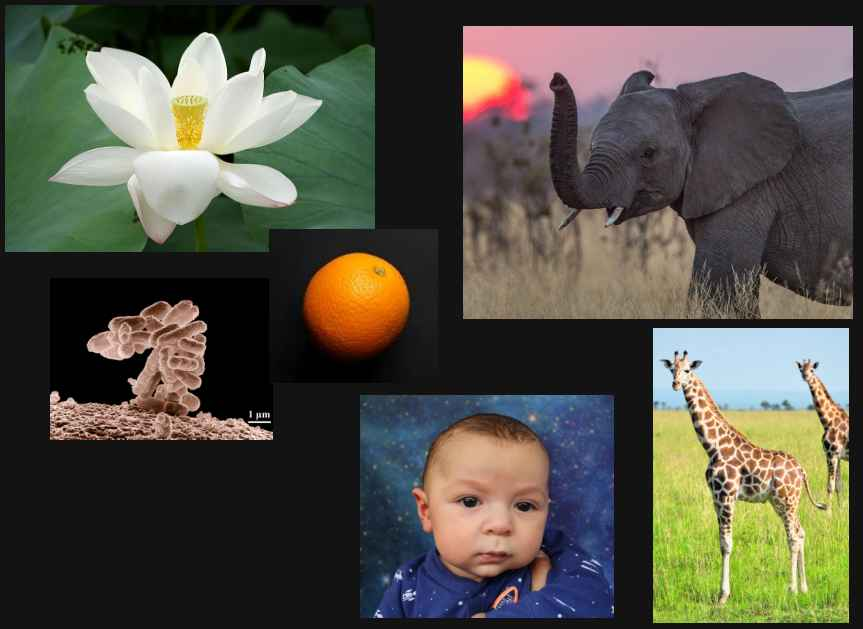
\includegraphics[width=0.8\textwidth]{WhatDoTheseSpeciesHaveInCommon}
	\end{center}
\end{figure}
They all contain \gls{gls:DNA}
and they share a genetic code
that programs for the different types
and arrangements of molecules
that make up their bodies.
Biologists have found a way
to utilize this information
in order to understand
the relationship between species.
As different as
all of these organisms are,
and as varied as
all of their genes may be,
all of Earth's known organisms
share a small group of genes
that encode for molecules
that have the same basic functions
in each of their cells.
These genes are critical
for cell replication,
meaning that the cells cannot persist
without these molecules.
So, it is important that
the sequences remain functional.
As a result, these genes tend to have
similar but not identical sequences
across different organisms.
Scientists can compare
how similar or how different
these similar sequences are
to create an ancestral tree
that demonstrates whether organisms
are more or less related to one another.
This is what is referred to
as a ''phylogenetic tree''.

Phylogenetic trees are hypotheses--they are not definitive facts.
\begin{itemize}
	\item The branching pattern
	in the phylogenetic tree
	illustrates how organisms are evolved
	from a list of common ancestors.
	
	\item If organisms are located
	near one another on the tree,
	it is very likely that those organisms
	are more closely related to one another
	or that they inherited those genes
	from a similar ancestor.
\end{itemize}

In a very broad sense,
a phylogenetic tree
that surveys relatedness
across many diverse groups
of organisms
may be thought of as a tree of life--Figure \ref{fig:TOL-5-3}--
a map that indicates
how every single organism
might be related to one another
going back billions of years to
the first ancestors of all life on Earth.

\begin{figure}[H]
	\begin{center}
		\caption[A phylogenetic tree may be thought of as a tree of life]{A phylogenetic tree that surveys relatedness across many diverse groups
			of organisms may be thought of as a tree of life}\label{fig:TOL-5-3}
		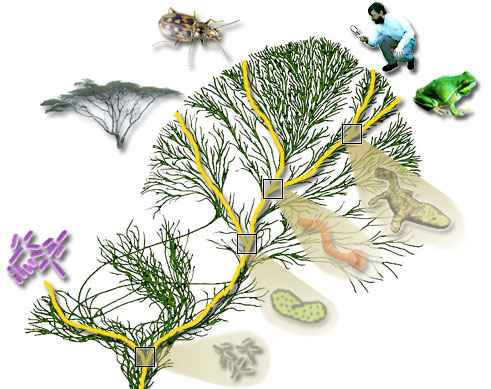
\includegraphics[width=0.8\textwidth]{TOL-5-3}
	\end{center}
\end{figure}


But, just because the origin of this tree
goes back billions of years,
it doesn't means that we have
all the information that is needed
to solve difficult problems
regarding life's origins and evolution.
Organisms that leave
recognizable fossils
are most from a group
called the "eukaryotes."
And, while millions of the these organisms
have been genetically cataloged,
over 99 percent of all species
that have ever lived on our planet
are estimated to have gone extinct -
meaning that our ability to extrapolate
backwards into the past is quite limited.
The limitations of sampling in our
available genetic and fossil records
severely limits our ability
to make inferences
about past relationships of organisms,
and genes... and genomes
to one another.
Nevertheless, the high degrees
of sequence similarities
across similar genes
found in all organisms
gives us ways in which we can
reconstruct the sequences
that were likely found in our ancestors.

\begin{itemize}
	\item $\approx 1.2$ million eukaryotes catalogued
	\item $\approx 8.9$ million eukaryotes present on Earth
	\item $>99\%$ of species have gone extinct thus severally limiting our starting pool
\end{itemize}

\subsubsection{Tree Thinking and phylogeny}


Let's take down to another level
a simple example of a phylogenetic tree.
The specific branching pattern
indicates the degree to which
current genes may resemble genes
that were found
in the common ancestors'
shared evolutionary history.
The genes that we can study
in extant organisms
are located near the ends of the branches
and are called ''leaves'' or ''tips''--Gigure \ref{fig:TreeTerminology}.
These are connected with branches
back to internal nodes
that represent the likely states
of shared ancestors.
The oldest node may be referred to
as a ''root'' of the tree.

\begin{figure}[H]
	\begin{center}
		\caption[Tree Terminology]{The genes that we can study
			in extant organisms
			are located near the ends of the branches
			and are called ''leaves'' or ''tips''--Gigure \ref{fig:TreeTerminology}.
			These are connected with branches
			back to internal nodes
			that represent the likely states
			of shared ancestors.
			The oldest node may be referred to
			as a ''root'' of the tree.}\label{fig:TreeTerminology}
		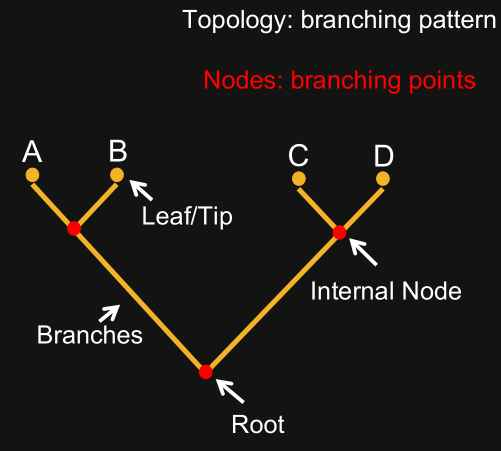
\includegraphics[width=0.6\textwidth]{TreeTerminology}
	\end{center}
\end{figure}

We can step sequentially backwards
through the different nodes
to investigate
what sequences or attributes
have been inherited from ancestors
or to estimate the timing
for the emergence
of newly evolved sequences or attributes.
From this, we can begin to develop
and investigate more specific questions
about the relatedness
of specific groups of organisms
or to estimate how ancestral traits
may have been modified
to yield the traits
of certain organisms today.

In examining even a simple tree,
there are many possible combinations
of sequence changes along the branches
that would fit the observed distribution
of sequences in existing organisms.
But, generally speaking,
in the lack of compelling evidence
to the contrary,
the simplest ways of gaining
and losing attributes -
such as requiring the fewest number
of genes, losses, additions -
that with the tree
will probably be the most accurate--Figure \ref{fig:PhylogenicTree}.

\begin{figure}[H]
	\caption[Generally the simplest tree will be most accurate]{Often there are many ways to model relationships, but generally the simplest will be most accurate.}\label{fig:PhylogenicTree}
	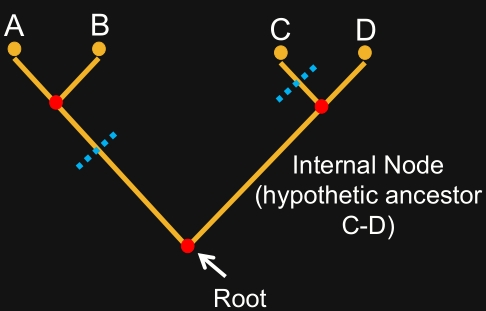
\includegraphics[width=0.9\textwidth]{PhylogenicTree}
\end{figure}


The steps that we use in this process
are straightforward--Figure \ref{fig:MolecularPhylogeneticsProtocol}.
\begin{itemize}
	\item First - sequences of the same genes
	from different organisms are collected.
	\item Next - these genes are aligned
	so that the key functional portions
	of each gene
	match up in the same column
	with one another.
	And, keep in mind that we can do
	this process for genomes as well.
	With more advanced programs,
	you can do this with
	multiple genes at once
	to get a more complete picture
	of how organisms might be related.
	\item Finally - trees are constructed using these genes.
	\item There are usually
	many different tree shapes
	or topologies that are possible
	using the same data set.
	So, different analyses are run to see
	which topologies require
	the fewest assumptions,
	or which best match up
	with the fossil record.
	
	\item It is only after a rigorous analysis
	of many different possible trees
	that phylogenies can be
	prudently interpreted
	and applied to evolutionary questions.
	
\end{itemize}

\begin{figure}[H]
	\caption{Molecular Phylogenetics Protocol}\label{fig:MolecularPhylogeneticsProtocol}
	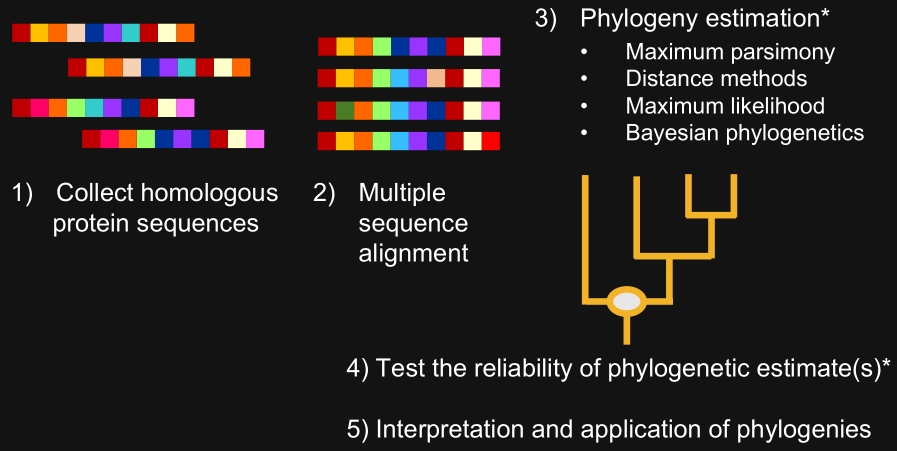
\includegraphics[width=0.9\textwidth]{MolecularPhylogeneticsProtocol}
\end{figure}
Though we have only run through
a quick survey
of how to construct phylogenetic trees,
there are many different applications
beyond just comparing the relatedness
of organisms to one another.
These applications look at
many different levels of biology,
from whole populations
down to individual proteins
and how they change over time.
Some other applications of phylogenetics
\begin{itemize}
	\item Classification and taxonomy of genes, proteins and species
	\item Comparative analysis and character evolution
	\item Predicting protein structure and function
	\item Investigating the history and demography of populations
	\item Studying the emergence and spread of viral and bacterial pandemics
	\item Searching for useful traits in related groups
\end{itemize}

Perhaps the most fundamental
contribution to origins studies
was the discovery that
all organisms on Earth
fall into one of three major groups--
bacteria, archaea and eukaryotes--Figure \ref{flg:the:big:picture}.
Before this magnificent discovery
by Carl Woese and George Fox in 1977,
organisms were classified into groupings -
mostly based on morphology.
And, there was almost no definitive way
to distinguish archaea
from bacteria at all
since they are both predominantly
small and single-celled.
This fundamental view
has helped to organize a focus
on the attributes and timing
of the last universal common ancestor -
or \gls{gls:LUCA}--
and has opened new questions
concerning the extent to which
\gls{gls:LUCA}'s emergence may actually be
pretty far removed from life's origins.
Based on the attributes
of all of its descendants,
it seems clear that \gls{gls:LUCA} was already
a very sophisticated organism
and many open questions remain
as to what must have been
an extensive pre-\gls{gls:LUCA} history
of emergence and evolutionary innovation.


\begin{figure}[H]
	\caption[Phylogenetic Tree of Life--The big picture]{Phylogenetic Tree of Life--The big picture\cite{wiki:tol:biology}}
	\label{flg:the:big:picture}
	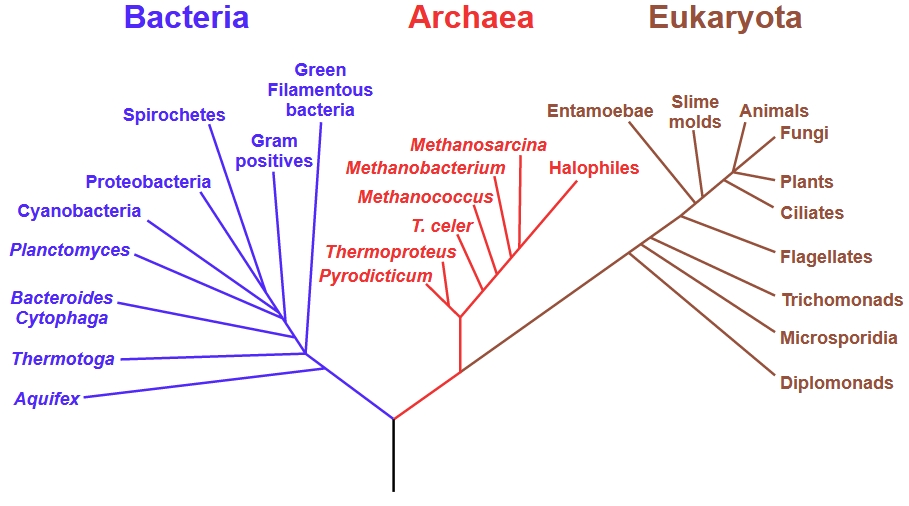
\includegraphics[width=0.9\textwidth]{TOL5}
\end{figure}

See \cite{hillis1996molecular,zuckerkandl1965molecules,williams2006assessing,woese2002evolution}

\subsection[A Deeper Dive into Phylogenetics]{A Deeper Dive into Phylogenetics--Andy Rominger}

We will be talking about:
\begin{itemize}
	\item How to statistically infer a phylogeny from data on Species living in the present;
	\item Why the Deep Past is so difficult to infer from this contemporary data.
\end{itemize}

\subsubsection{How to Infer a Phylogeny}
We are going to focus on step 3 of Figure \ref{fig:MolecularPhylogeneticsProtocol}, finding the evolutionary process leading to the data we have. We start with \gls{gls:homologous} sequences, and we want to infer the speciation, extinction, and passing genes on to daughter lineages. This process also involves mutation, because the changes in \gls{gls:DNA} are what allow us to infer the past. Figure  \ref{fig:InferringPhylogeny} therefore shows a mutation rate matrix. 

We have transition rates, topology, and sequence data--Figure \ref{fig:InferringPhylogeny1}--and we want to choose transition rates and a topology to \textit{maximize the likelihood}--Figures \ref{fig:InferringPhylogeny2}. 

\begin{figure}[H]
	\caption{Inferring a phylogeny}\label{fig:InferringPhylogeny}
	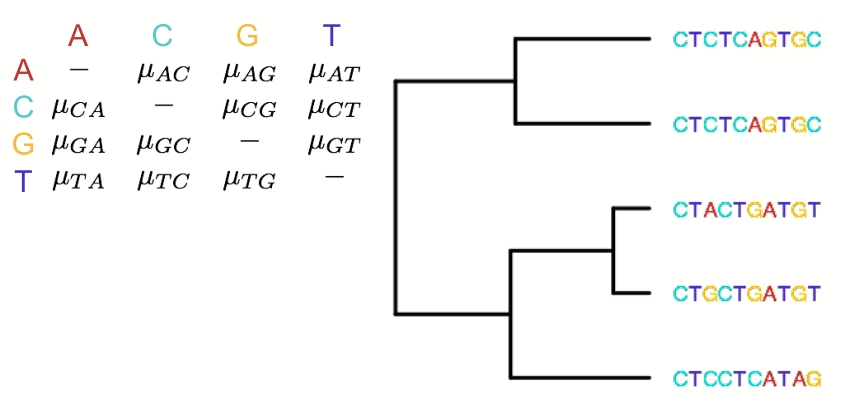
\includegraphics[width=0.9\textwidth]{InferringPhylogeny}
\end{figure}

\begin{figure}[H]
	\caption{Goal: find the process leading to the data}\label{fig:InferringPhylogeny1}
	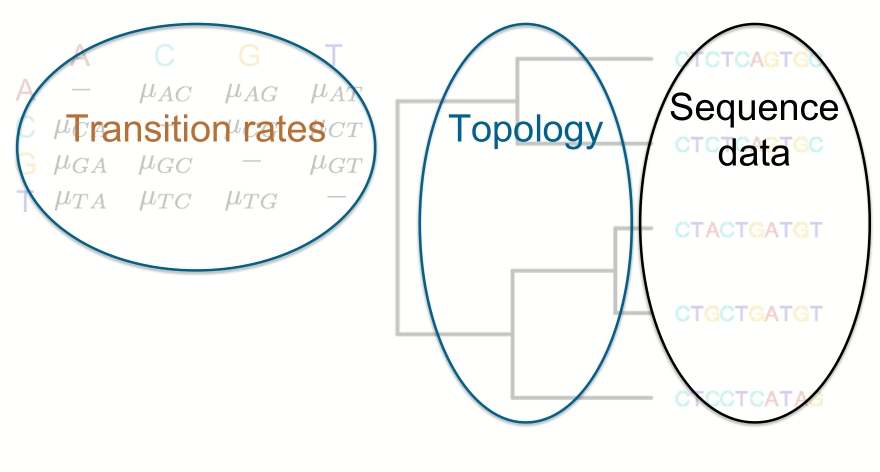
\includegraphics[width=0.9\textwidth]{InferringPhylogeny1}
\end{figure}

\begin{figure}[H]
	\caption{Maximize Likelihood}\label{fig:InferringPhylogeny2}
	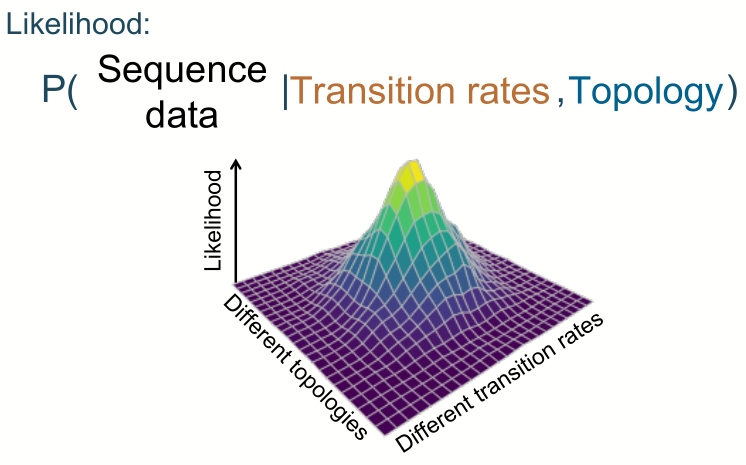
\includegraphics[width=0.9\textwidth]{InferringPhylogeny2}
\end{figure}

\begin{itemize}
	\item The inference procedure that we have described is called Maximum Likelihood Inference\cite{huelsenbeck1997phylogeny}--Figure \ref{fig:InferingPhylogeny}
	\item Bayesian inference: traversing the complex topology and
	rate matrix space lends itself to Bayesian algorithms\cite{huelsenbeck2001mrbayes,huelsenbeck2001introduction}
\end{itemize}
\begin{figure}[H]
	\caption[Inferring Phylogeny]{Inferring Phylogeny: in practice topologies are not this simple.}\label{fig:InferingPhylogeny}
	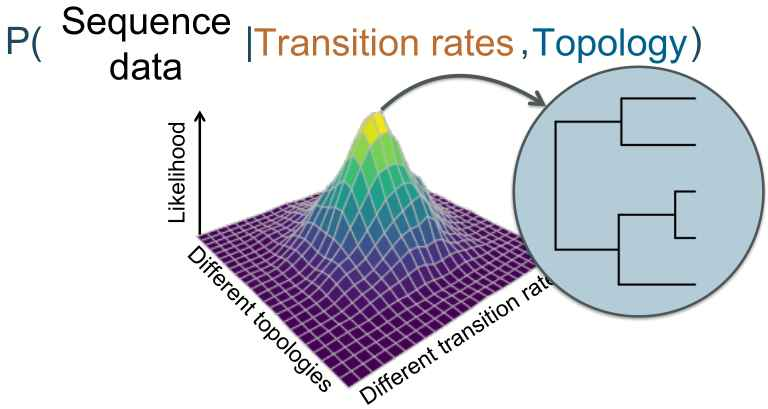
\includegraphics[width=0.8\textwidth]{InferingPhylogeny}
\end{figure}
Two other procedures have been used historically:
\begin{itemize}
	\item Parsimony
	\item Distance based inference
\end{itemize}

\subsubsection{Why is the Deep Past so difficult to infer?}
Caveats: Inferring the past it hard.
\begin{itemize}
	\item Unrooted phylogeny
	\item \gls{gls:TOL} has no outgroup.
	\item Time Calibration
	\item \Gls{gls:long:branch:attraction}
	\item What genetic information goes back to LUCA?
\end{itemize}

Unrooted phylogeny arises because mutation process is reversible in our models--Figure \ref{fig:unrooted:phylogeny}. We don't know where the ultimate ancestor is, and how it had led to the present tips. This is why the Banfield Tree of Life has no root--Figure \ref{fig:banfield:tol}.
 
\begin{figure}[H]
	\caption[Unrooted phylogeny arises because mutation process is reversible]{Unrooted phylogeny arises because mutation process is reversible in our models}\label{fig:unrooted:phylogeny}
	\begin{subfigure}[b]{0.45\textwidth}
		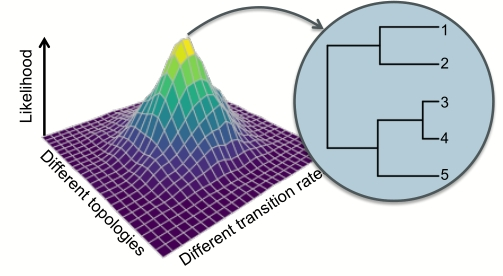
\includegraphics[width=\textwidth]{InferringPastHard1}
	\end{subfigure}
	\begin{subfigure}[b]{0.45\textwidth}
		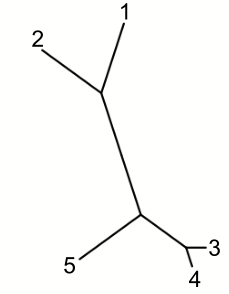
\includegraphics[width=\textwidth]{InferringPastHard2}
	\end{subfigure}
\end{figure}

\begin{figure}[H]
	\caption[Banfield Tree of Life]{Banfield Tree of Life\cite{hug2016new}}\label{fig:banfield:tol}
	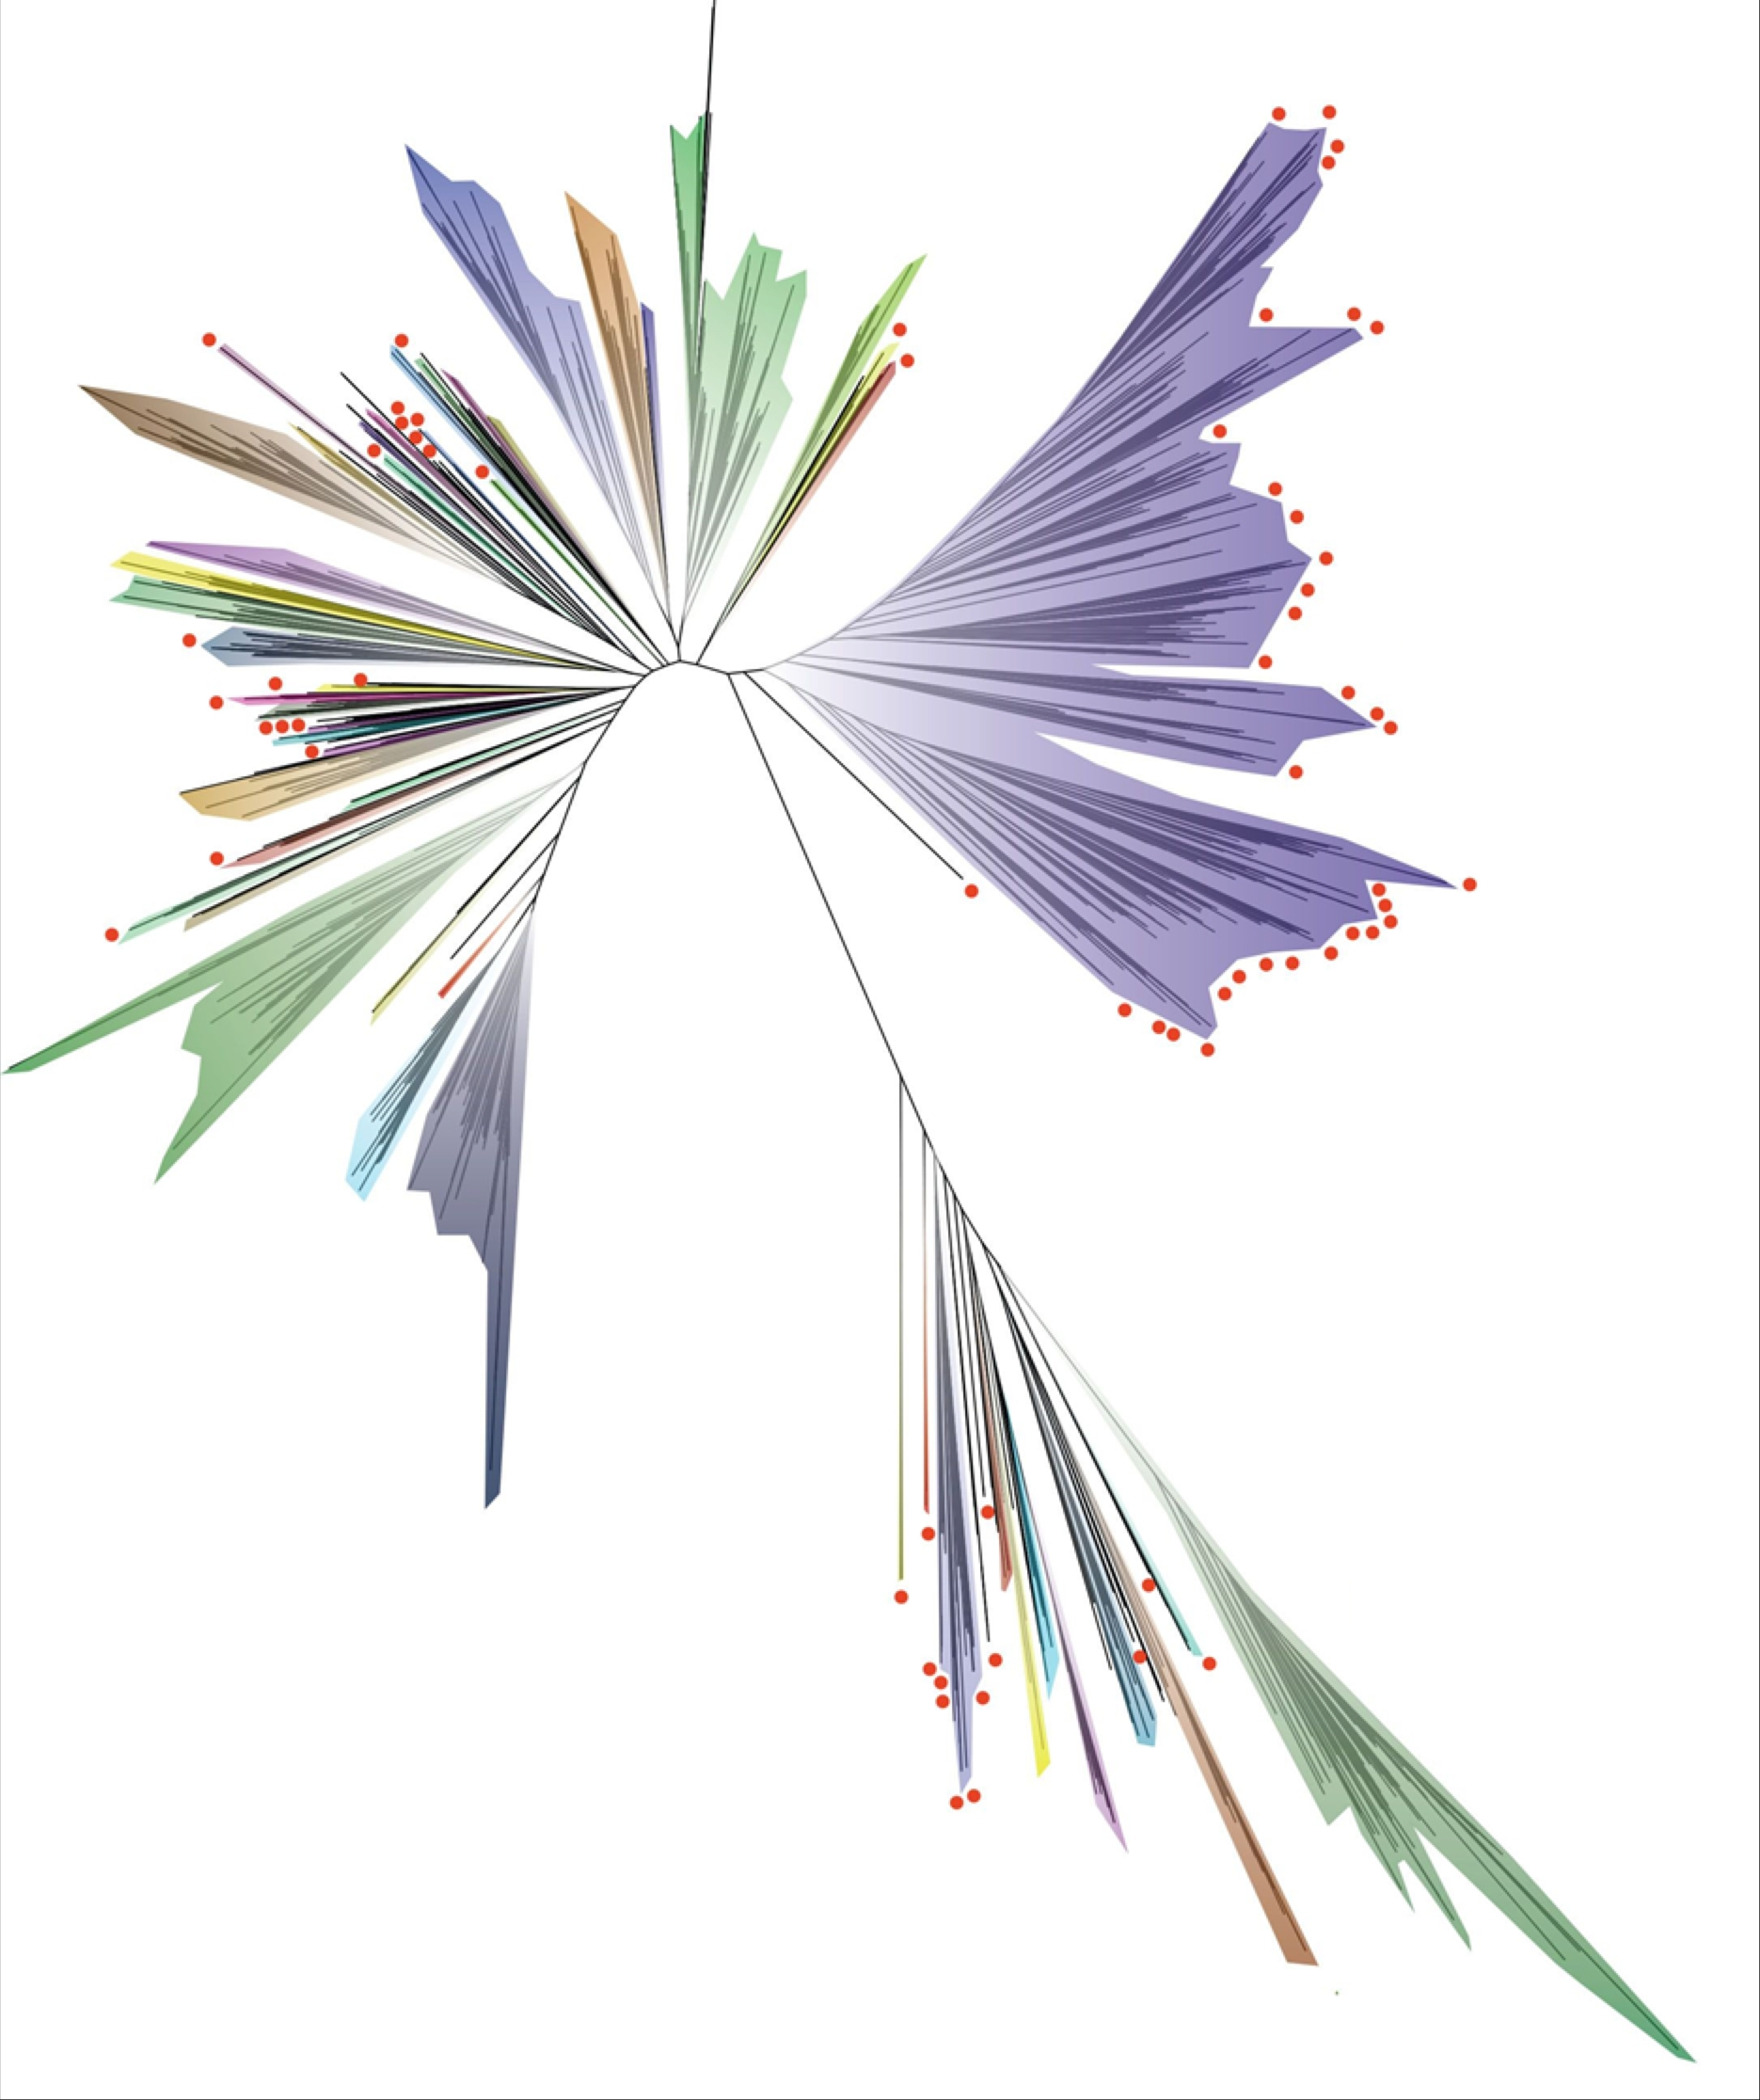
\includegraphics[width=0.9\textwidth]{TOL4}
\end{figure}

The best method we have for rooting a tree is to use an \gls{gls:outgroup}. We can add a new group to the tree of mammals--Figures \ref{fig:bird:without:outgroup} and \ref{fig:bird:outgroup}. In Figure \ref{fig:bird:outgroup} the root is where the bird connects to the mammals: we have added temporal directionality to the tree.But the \gls{gls:TOL}, by definition, has no \gls{gls:outgroup}!

\begin{figure}[H]
	\caption{Adding an Outgroup to the Tree of Mammals}
	\begin{subfigure}[t]{0.3\textwidth}
		\caption{An unrooted tree of mammals}\label{fig:bird:without:outgroup}
		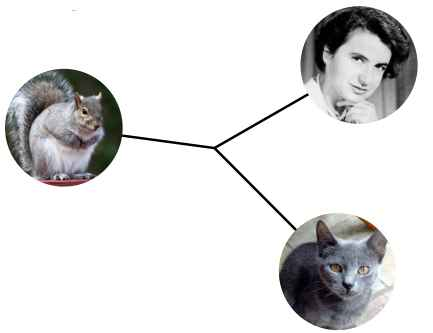
\includegraphics[width=0.9\textwidth]{WithoutOutgroup}
	\end{subfigure}
	\begin{subfigure}[t]{0.3\textwidth}
		\caption{Using a Bird as an Outgroup}\label{fig:bird:outgroup}
		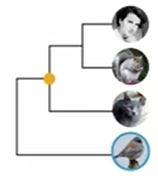
\includegraphics[width=0.9\textwidth]{Outgroup}
	\end{subfigure}
	\begin{subfigure}[t]{0.3\textwidth}
		\caption{Tree of Mammals (plus outgroup)}\label{fig:bird-mammals}
		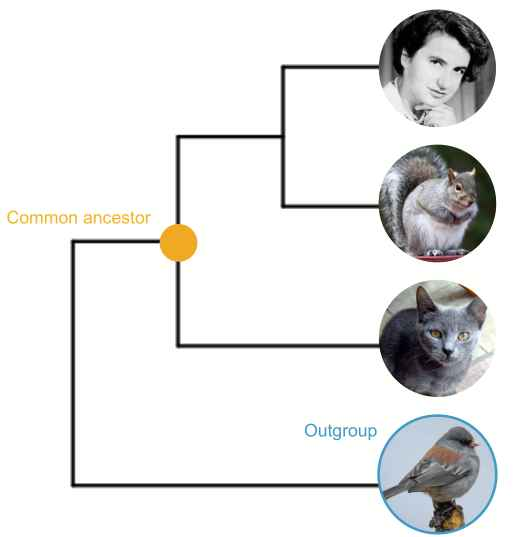
\includegraphics[width=0.9\textwidth]{bird-mammals}
	\end{subfigure}
\end{figure}

Another problem is that rate heterogeneity means that mutations are not clock like\cite{sanderson2003r8s,smit2007evolutionary}. Time in a phylogeny is measured in substitutions, not in years. Since the rate of mutation varies across lineages and across Earth's history, mutation events don't tell us the time on each branch. So species in the Banfield Tree of Life--Figure \ref{fig:banfield:tol}-- don't line up. We need additional information to calibrate substitution events against time.
\begin{itemize}
	\item We may be able to assign times from the fossil record--Figure \ref{fig:calibrating-time}.
	\item In some cases we \textit{do} know the mutation rate and can use it like a clock.
\end{itemize}

\begin{figure}[H]
	\caption[We must calibrate 	phylogenies with independent data]{We must calibrate 	phylogenies with independent data, 	e.g. the fossil record, known mutation rates for specific groups.}\label{fig:calibrating-time}
	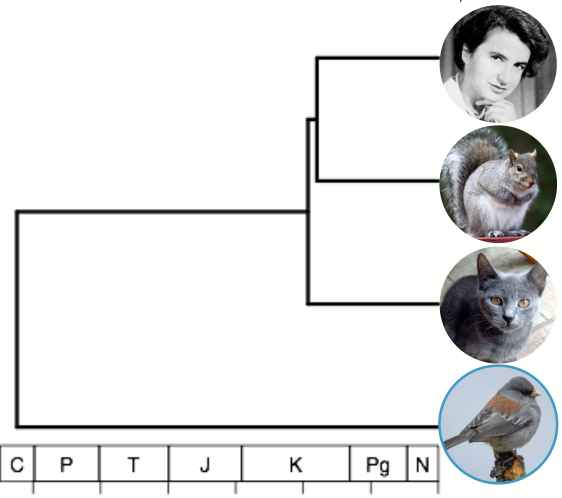
\includegraphics[width=0.6\textwidth]{calibrating-time}
\end{figure}
Long branches attract each other\cite{philippe2005heterotachy}--Figure \ref{fig:long:branches}. The longer a lineage has been evolving, the more time there has been for mutations to accrue, and divergent sequences can, by chance, appear convergent, or else can evolve totally away. So our inference methods end up clustering data

\begin{figure}[H]
	\caption[Long branches attract each other]{Long branches attract each other. Where to group the lowest sequence?}\label{fig:long:branches}
	\begin{subfigure}[b]{0.3\textwidth}
		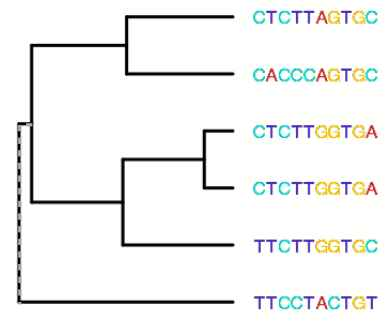
\includegraphics[width=\textwidth]{LongBranchAttraction0}
	\end{subfigure}
	\begin{subfigure}[b]{0.3\textwidth}
		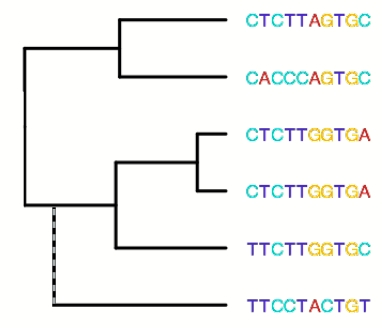
\includegraphics[width=\textwidth]{LongBranchAttraction1}
	\end{subfigure}
	\begin{subfigure}[b]{0.3\textwidth}
		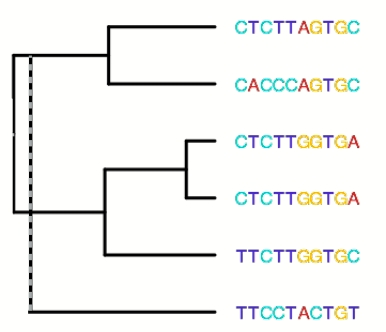
\includegraphics[width=\textwidth]{LongBranchAttraction2}
	\end{subfigure}
\end{figure}

 What genetic information goes back to LUCA? Figure \ref{fig:back_to_LUCA} illustrates that billions of years separate bacterial and human DNA. All life needs to translate DNA into proteins, and all of life uses ribosomes to do this. Therefore Ribosomal RNA and protein genes are exactly the genes that we can use to infer these deep phylogenetic relationships\cite{quast2012silva} and Figure \ref{fig:Ribosome-5-3-2}.
 
 \begin{figure}[H]
 	\caption{What genetic information goes back to LUCA? }
 	\begin{subfigure}[t]{0.45\textwidth}
 		\caption{Billions of years separate bacterial and human DNA}
 		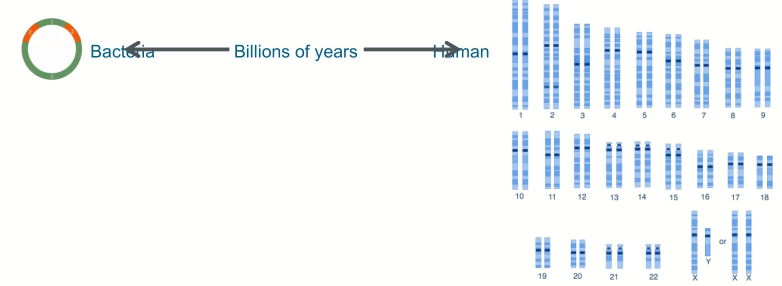
\includegraphics[width=\textwidth]{LUCA_what_goes_back}\label{fig:back_to_LUCA}
 	\end{subfigure}
 	\;\;\;
	 \begin{subfigure}[t]{0.45\textwidth}
	 	\caption{Ribosomal RNA and protein genes}\label{fig:Ribosome-5-3-2}
	 	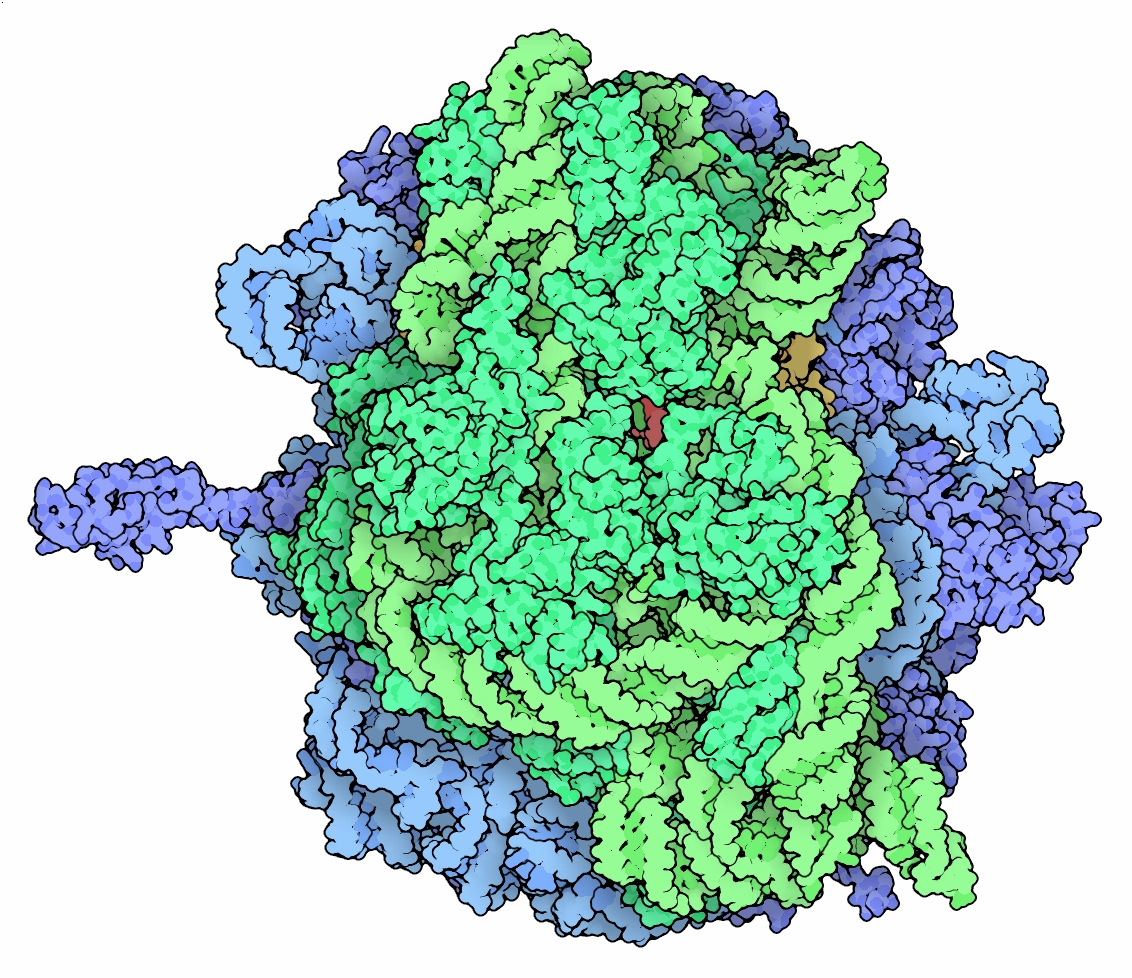
\includegraphics[width=0.45\textwidth]{Ribosome-5-3-2}
	 \end{subfigure}
 \end{figure}

Given these caveats, it is remarkable that different research groups have been able to reconstruct such detailed phylogenies for all life, and many of these phylogenies are robust because they have gone to great lengths to overcome these challenges.


\section[Macroscopic Theories in Biology]{Macroscopic Theories in Biology--Chris Kempes}
 
One of the main questions from this course is: which aspects of extant life are general, and which are arbitrary? If we look at the diversity of life on this planet:
\begin{itemize}
	\item how much of what we see is peculiar to the trajectory of life on our own planet?
	\item how much would be true of life anywhere?
\end{itemize}

This matters not just for exobiology, but also for understanding what early life might have looked like, and the origin of life in general (not just our own planet).

In this course we have covered:
\begin{itemize}
	\item Laws of chemistry
	\item General processes of natural selection
	\item Laws of physics
\end{itemize}

\subsection{Are there Laws of Life?} 

There are certainly laws of physics and chemistry that apply to life, but are there distinct laws of life? We will talk about not only how the laws of physics and chemistry are coupled to the laws of life but also about how, once you have a particular biological structure, that determines a particular law of life. That law of life is about the evolutionary history that has brought you to a particular structure, and how that structure connects to the fundamental laws of physics, chemistry, and evolution.

What do we mean by a law? The most well know example is Newton's Law of Gravitation:
\begin{align*}
	F =& \frac{G m_1 m_2}{r^2} \numberthis \label{eq:newton}
\end{align*}

This holds anywhere in the Universe, it holds for any two masses, and any distance between them. We can understand all sorts of planetary relationships based on this one law.

\begin{itemize}
	\item If we were trying to verify the Law experimentally, we might see data like Figure \ref{fig:Newton:Experimental}
	\item \emph{Maybe} we'd observe a fundamental shift in physics for very small distances--Figure \ref{fig:Newton:Shift}--perhaps a quantum effect. 
\end{itemize}
\begin{figure}[H]
	\caption{Newton's Law of Universal Gravitation}
	\begin{subfigure}[t]{0.45\textwidth}
		\caption{If we were trying to verify the Law experimentally, we might see data like this (masses have been randomized)}\label{fig:Newton:Experimental}
		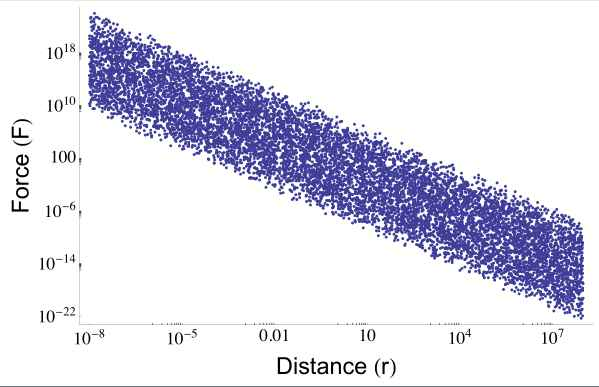
\includegraphics[width=\textwidth]{Newton}
	\end{subfigure}
	\;\;\;
	\begin{subfigure}[t]{0.45\textwidth}
		\caption{\emph{Maybe} we'd observe a fundamental shift in physics for very small distances(contrived example.)}\label{fig:Newton:Shift}
		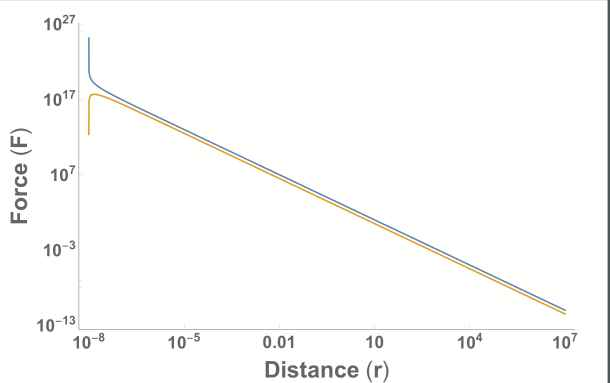
\includegraphics[width=\textwidth]{Newton2}
	\end{subfigure}
\end{figure}

The question becomes: \begin{itemize}
	\item are there laws in biology analogous to (\ref{eq:newton})? 
	\item what do they look like?
	\item where do they come from?
\end{itemize}

Why should we expect that there are laws in biology at all? Organisms evolve within the bounds of chemistry and physics; you should never see an organism disobeying any of the known rules of chemistry or physics. At a more subtle level, as organisms evolve they may be able to optimize their physiology with respect to one or more physical constraints. they may see some constraint as a detriment to \gls{gls:fitness}: evolution may select for organisms that are able to do a better job of dealing with the constraint in a way that makes them more fit--more likely to reproduce\cite[Chapter 10, An Agony in Five Fits]{dawkins1982extended}. They might, over time, optimize according to the most dominant constraints given their physiology.

\subsection{Examples of Laws of Life}

\subsubsection{Mammals}

We will start with mammals. This is a very advanced place to start: these are some of the most complicated organism we know, that have had the most evolutionary time to reach the body plan they have. We'll look at Body mass and \gls{gls:BMR}.  Figure \ref{fig:allometric:scaling} shows the Relationship between peak post-feeding resting metabolic rate and body mass for mammals--an approximate power law with an exponent of $\frac{3}{4}$. Since this isn't a simple proportionality is shows that there may be something interesting going on: despite all this diversity of mammals, despite all their diverse strategies, there is this relationship, which we might call a law for mammals. What physics leads to this?

\begin{figure}[H]
	\caption[Relationship between BMR and body mass]{Relationship between peak postfeeding resting metabolic rate and body mass-\cite{white2005allometric}}\label{fig:allometric:scaling}
	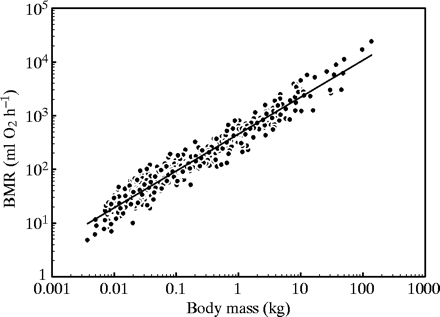
\includegraphics[width=0.9\textwidth]{WhiteSeymour}
\end{figure}

Geoffrey West, Jim Brown and Brian Enquist\cite{west1997general} have shown that if you: \begin{itemize}
	\item consider the fractal vascular structure of mammals and plants--Figure \ref{fig:FractalBranching};
	\item optimize it so it fills space and brings resources to all cells--or, in the case of plants, if we  fill canopy with leaves to so solar radiation can be absorbed;
	\item think about hydrodynamic resistance, and consider the need to not buckle under the force of gravity in the case of a tree, and put all these physical constraints together;
	\item minimize the energy required to distribute resources;
\end{itemize}
Then the optimization prodicts the $\frac{3}{4}$ exponent: Body Plan + Constraints$\rightarrow$Law of Life.

\begin{figure}[H]
	\caption{Power Law follows from the fractal vascular structure of mammals.}\label{fig:FractalBranching}
	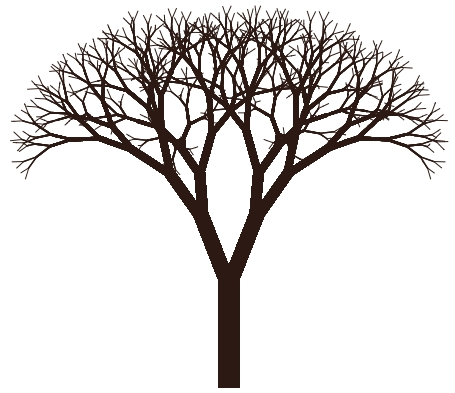
\includegraphics[width=0.9\textwidth]{FractalBranching}
\end{figure}

This is a  way to take a body plan, couple it with constraints, and then predict some emergent law for a particular class of organisms.

\subsubsection{Example of a Fundamental Constraint}

The foregoing is a very complicated example, but there are examples of these types of laws at all scales of life, and there are some that connect to very fundamental constraints. We will discuss one example in the next section, but be aware that there is a very rich literature on different physical constraints.

Diffusion to a simple spherical cell drifting passively. Cell is living in a still fluid filled with nutrients, and we want to know how nutrients diffuse to cell. We will solve the diffusion equation\footnote{\cite[Lecture 3.8: Systematics and Limits of Metabolic Rates]{sfi2020}}, and assume that the cell uses all of nutrients, so concentration at surface is held at zero.

\begin{align*}
	C(r) =& C_{\infty}\big(1 - \frac{r_c}{r}\big)\text{, where}\\
	r_c=& \text{ radius of cell}\\
	C_{\infty} =& \text{ concentration at infinity}\\
	C(r) =& \text{ concentration at distance r. Then the flux in is given by}\\
	J(r) =& D\frac{\partial C}{\partial R} \text{, where $D$ is the diffusion constant}\\
	  =& D C_{\infty} \frac{r_c}{r^2}\text{. We can compute the total uptake of nutrient}\\
	U =& 4 \pi r_c^2 J(r_c) \\
	=& 4 \pi\cancel{ r_c^2} D C_{\infty} \frac{r_c}{\cancel{r_c^2}}\\
	=&4 \pi D C_{\infty} r_c 
\end{align*}

This gives us a variety of physical and metabolic limitations, since no rate process within the cell can use the nutrient more quickly than $U$, so all processes must scale with $r$ at this rate or more slowly. If process want to go faster than $U$, the fluid needs to be disturbed, or the cell needs to move. This gives a very particular physiological outcome.

\subsubsection{Bacterial Physiology}

In Chris's own work, his team has looked at cell physiology across the entire range of cell sizes and found they can predict various volumes through power laws--Figure \ref{fig:BacterialPhysiology}. This shows the tradeoffs between quantities for small and large bacteria.
\begin{itemize}
	\item at the small end the cell runs out of space for DNA and protein;
	\item at the large end it runs out of space for all the RNA components.
\end{itemize}

\begin{figure}[H]
	\caption[The variation of component size with cell size]{The variation of component size with cell size; it \textit{bounds} the cell size: at the large end and small end the cell runs out of space for fundamental components.\cite{kempes2016evolutionary}}\label{fig:BacterialPhysiology}
	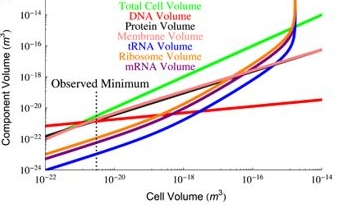
\includegraphics[width=0.9\textwidth]{BacterialPhysiology}
\end{figure}

This set of physiological laws comes with a particular concept of optimization and physiological tradeoffs. We might play with how these laws might vary and create an abstract physiological space and look at all physiological possibilities. This might be more relevant in a variety of early life contexts before life reaches to degree of optimization discussed in this Section


See also \cite{kempes2011predicting}.

\section{Selection-- Michael Lachmann}

\subsection{The Origin of Species}
Charles Darwin laid out a careful and well thought argument--''A naturalist, reflecting on the mutual affinities of organic beings, on their embryological relations, their geographical distribution, geological succession, and other such facts, might come to the conclusion that each species had not been independently created, but had descended, like varieties, from other  species''\cite{darwin1859origin}.

Darwin presented a phylogenetic Tree--\ref{fig:TOL:Darwin}. A modern view, Figure \ref{fig:TOL:Modern} is more like a web than a tree. Large parts of our genome came from viruses, and our bodies are full of bacteria and other symbionts. Some may stay for only a few weeks, but others might transmit vertically through the lineage. Out mitochondria, for example, who are responsible for out being able to live with oxygen and use it, were once free living, but, today, live in each cell and reproduce with it.

\begin{figure}[H]
	\caption{Two views of the Tree of Life}
	\begin{subfigure}[b]{0.45\textwidth}
		\caption{Darwin's TOL\cite{darwin1859origin}}\label{fig:TOL:Darwin}
		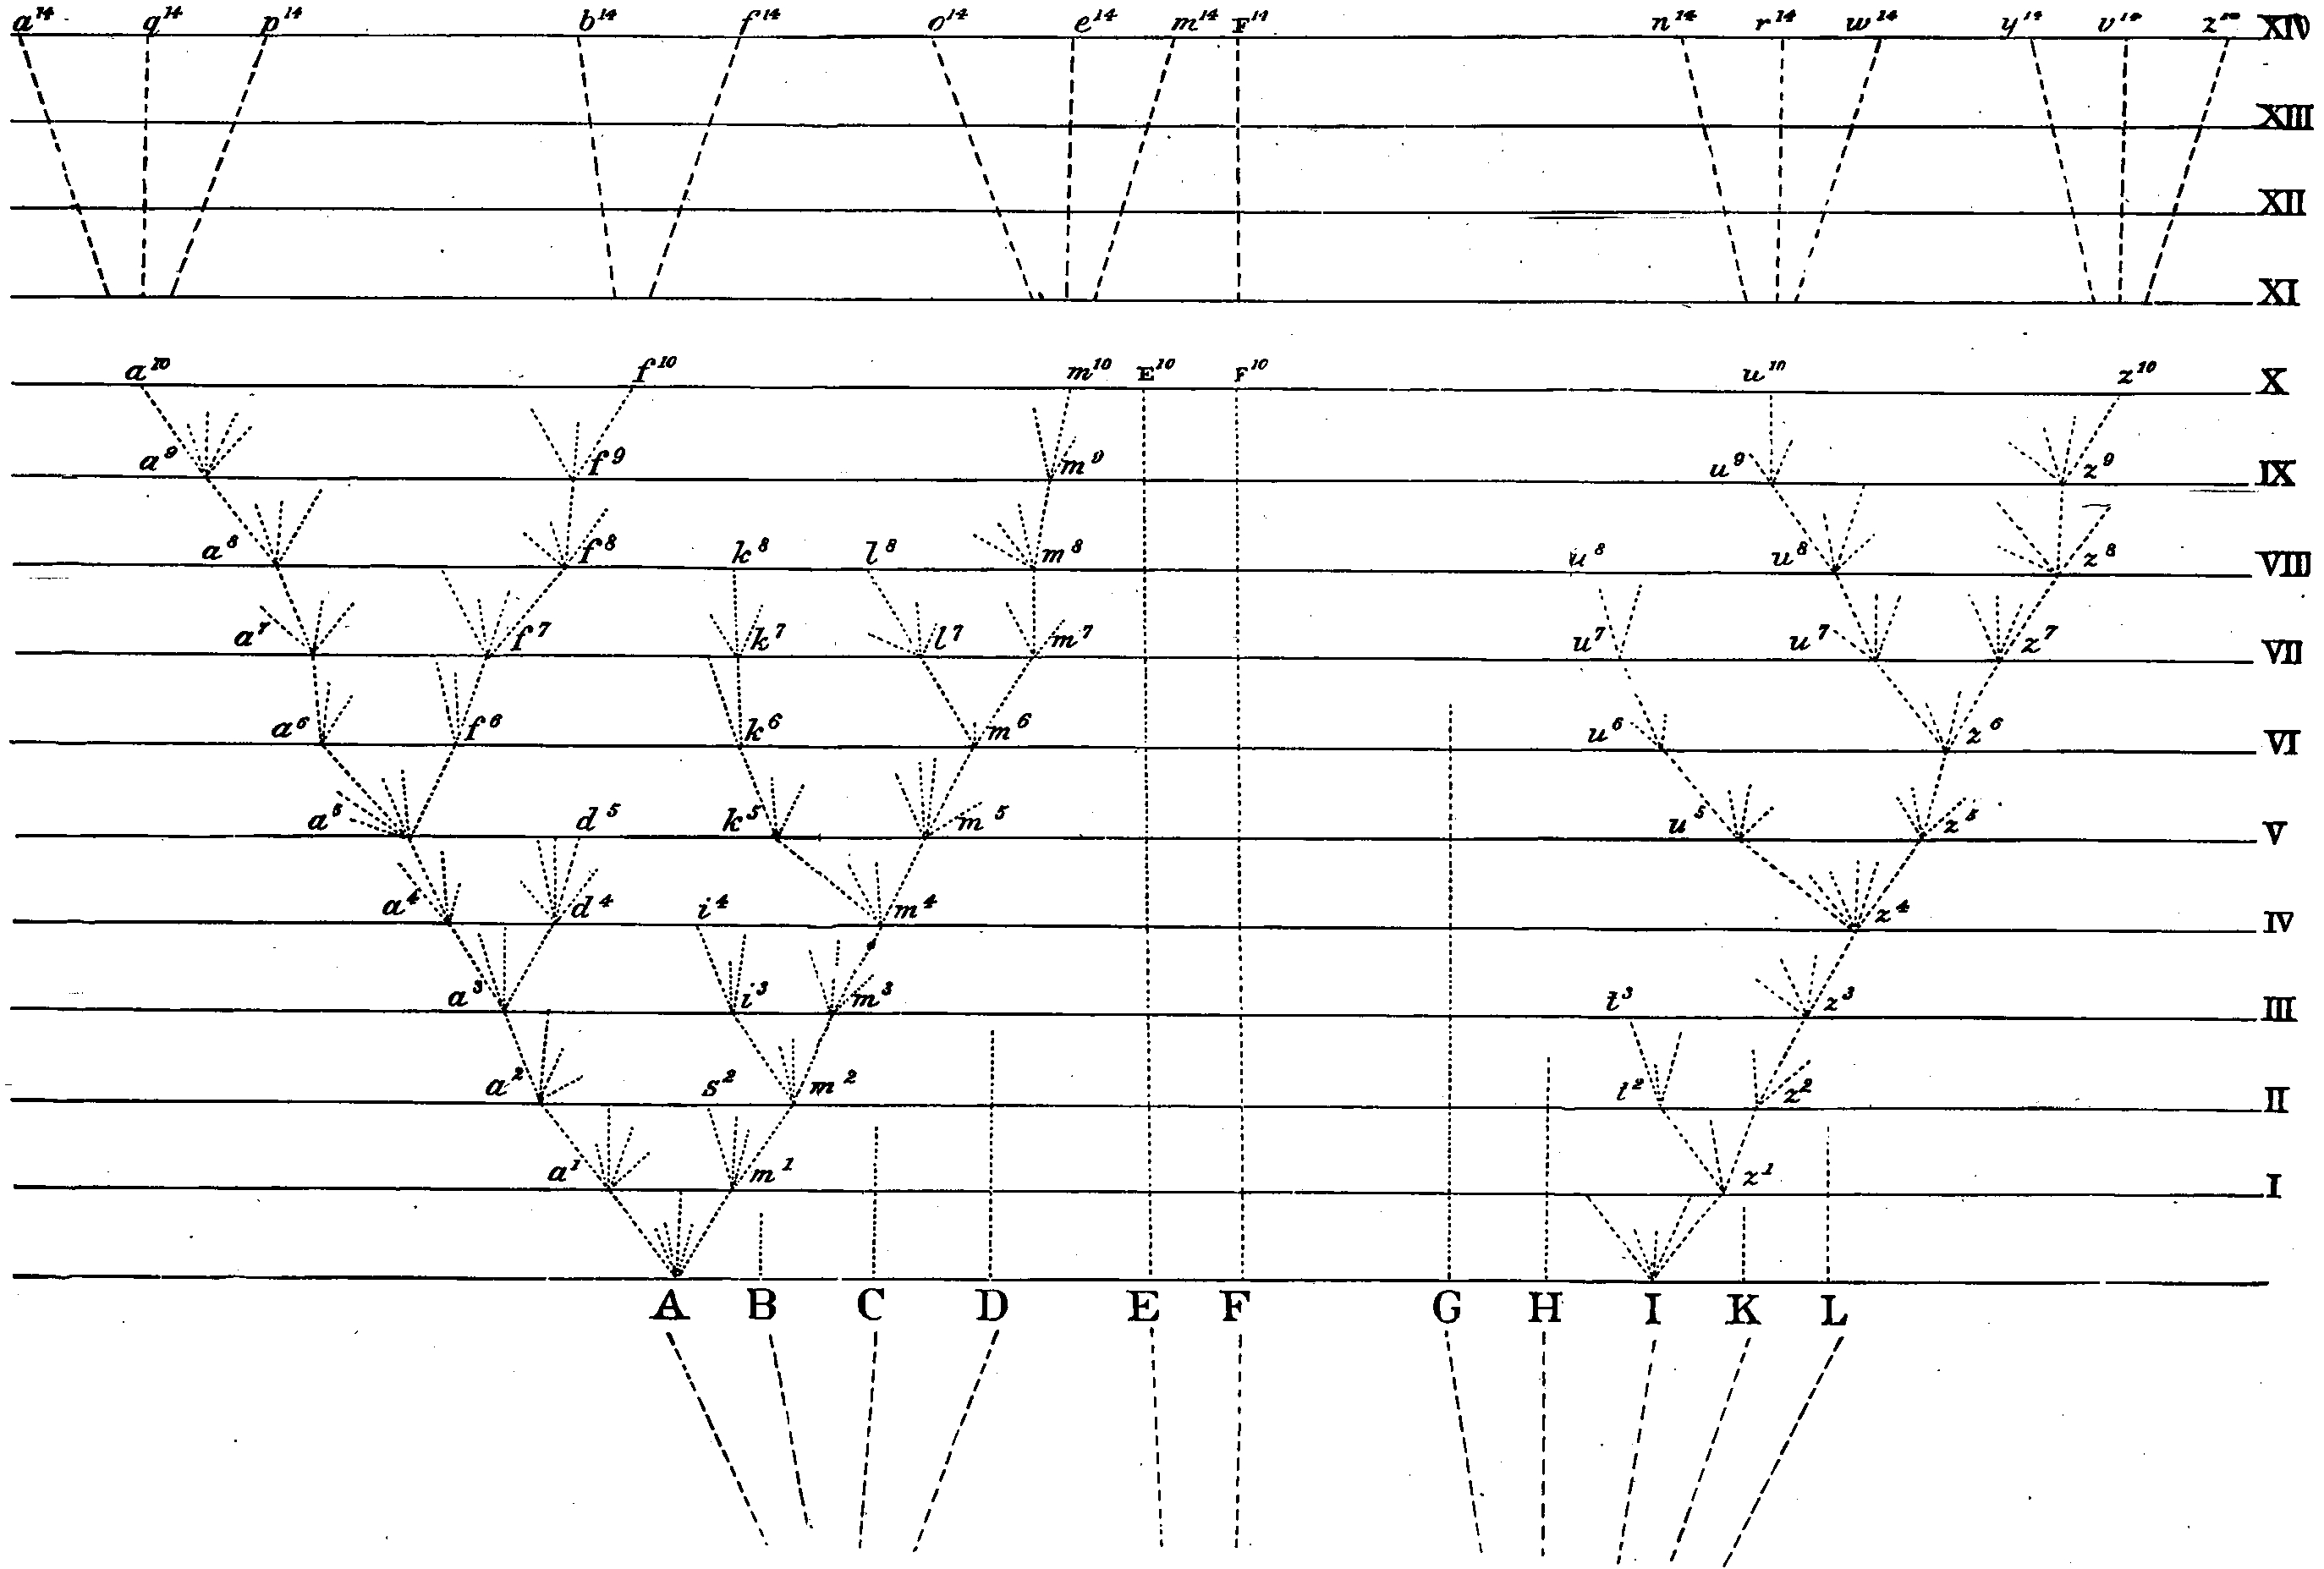
\includegraphics[width=\textwidth]{TOL_Darwin}
	\end{subfigure}
	\begin{subfigure}[b]{0.45\textwidth}
		\caption{Modern TOL}\label{fig:TOL:Modern}
		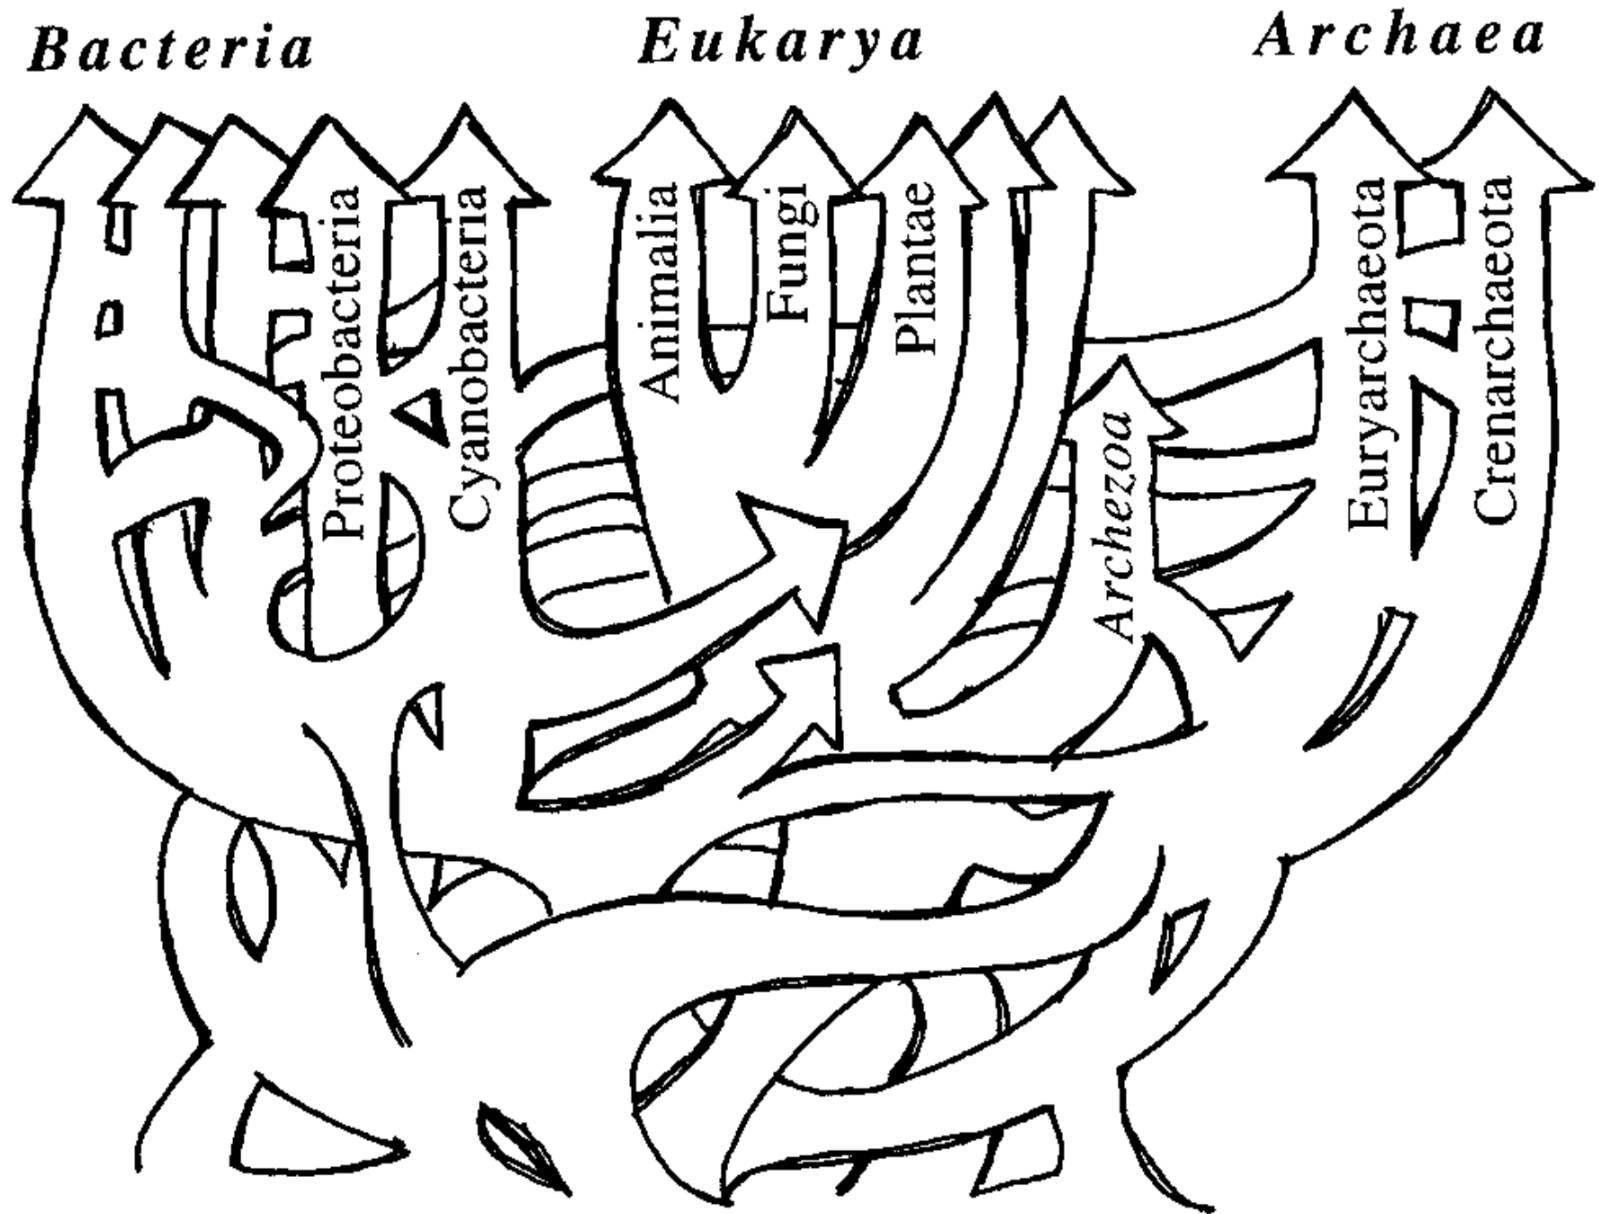
\includegraphics[width=\textwidth]{TOL-5-6}
	\end{subfigure}
\end{figure}

Darwin made the point that species evolved from one another, but: ''Nevertheless, such a conclusion, even if well founded, would be unsatisfactory, until it could be shown how the innumerable species inhabiting this world have been modified, so as to acquire that perfection of structure and coadaptation which most justly excites our admiration''--\cite{darwin1859origin}.

\subsection{How do species acquire that perfection of structure?}
How do species acquire that perfection of structure? There are three parts.
\begin{itemize}
	\item Variation: individuals in the population differ from one another.
	\item Inheritance: the variation is passed from one generation to another.
	\item Selection: the variations affect the survival of some individuals.
\end{itemize}

For example, consider a butterfly population with differences in colour, some darker, some lighter, living on black trees--Figure \ref{fig:SelectionMoths0}. Those whose colour blends in with the tree survive better; \emph{ if colour is inherited}, the differential survival will lead to an increase of the frequency of dark moths in the population--Figures \ref{fig:SelectionMoths1} and  \ref{fig:SelectionMoths2}. If this continues over many generations, only black butterflies will remain, and we will run out of variation in the population, and the butterflies will not be able to adapt to a new tree colour. Genetic mutation continually inject new variation onto the population, allowing further evolution
\begin{figure}[H]
	\caption{Example of natural selection--light and dark butterflies}\label{fig:SelectionMoths}
	\begin{subfigure}[t]{0.3\textwidth}
		\caption{Butterfly population with differences in colour}\label{fig:SelectionMoths0}
		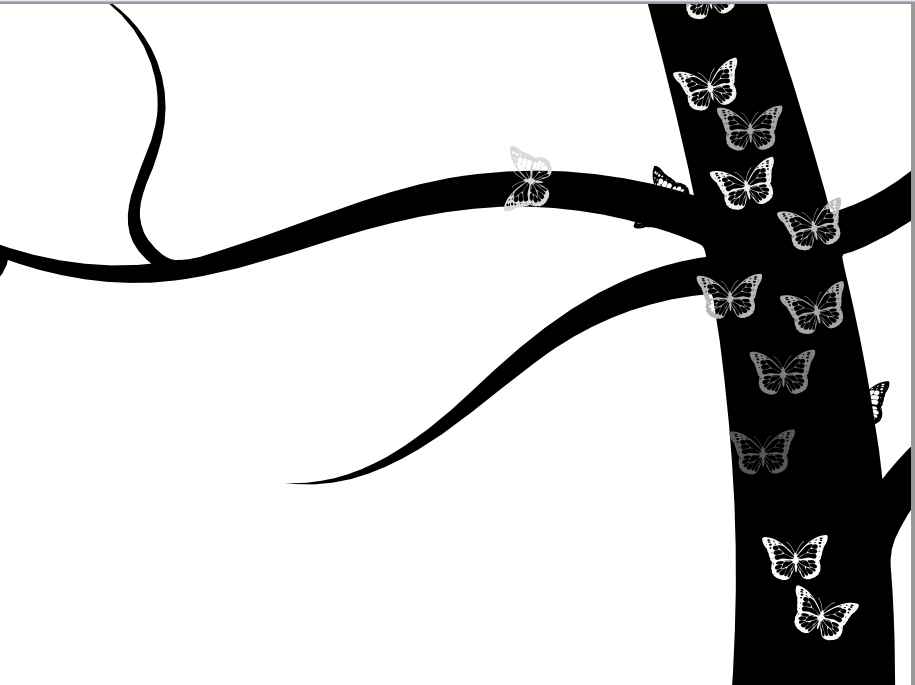
\includegraphics[width=0.8\textwidth]{SelectionMoths}
	\end{subfigure}
	\;\;\;
	\begin{subfigure}[t]{0.3\textwidth}
		\caption{Those whose colour blends in with the tree survive better.}\label{fig:SelectionMoths1}
		\includegraphics[width=0.8\textwidth]{SelectionMoths1}
	\end{subfigure}
	\;\;\;
	\begin{subfigure}[t]{0.3\textwidth}
		\caption{ \emph{ If colour is inherited}, the frequency of dark moths in the population will increase}\label{fig:SelectionMoths2}
		\includegraphics[width=0.8\textwidth]{SelectionMoths2}
	\end{subfigure}
\end{figure}

The example examined survivability, but, in addition to survival, other traits are selected in populations, such as number of offspring produces, mating success, sexual selection--Figure \ref{fig:BrightBird}. What exactly is selected for? Some have looked at number of children, grand-children, etc. The trait that is actually selected is long-term survival of the lineage in question, as compared to other lineages.

\begin{figure}[H]
	\caption[What exactly is selected for?]{In addition to survival, other traits are selected in populations, such as number of offspring produces, mating success, sexual selection. What exactly is selected for?}\label{fig:BrightBird}
	\includegraphics[width=0.8\textwidth]{BrightBird}
\end{figure}

\subsection{Variational versus Transformational Processes}
Figure \ref{fig:SelectionMoths0} is a variational process. The average colour changed, not because of a change in individual butterflies, but because some butterflies survived more than others. Compare with a population of chameleons, where each chameleon will change colour if you put it on a dark tree--Figure \ref{fig:chamelion}.
\begin{figure}[H]
	\begin{center}
		\caption[ Compare with a population of chameleons]{ Compare with a population of chameleons, where each chameleon will change colour if you put it on a dark tree.}\label{fig:chamelion}
		\includegraphics[width=0.6\textwidth]{chamelion}
	\end{center}
\end{figure}

Consider memes.
\begin{itemize}
	\item I can hear a joke and think how to make it funnier so it will spread better
	\item or maybe jokes that seem funnier spread better
\end{itemize}

In both cases we end up with funny jokes: in the first can it depends on my ability to transform jokes, in the other we have differences in spreading.

\subsection{The Price Equation}

The \gls{gls:price:equation}\cite{gardner2020price,price1970selection,frank2012natural} is a nice way to look at these two processes. It looks at the change of something in the population, such as brightness of wing colour or funniness of jokes,  when something happens to a population, and a generation passes, or maybe just a day; some individuals survive, some reproduce. We look at the difference in the property over this time.
\begin{align*}
	\Delta Z =& \frac{Cov(Z,W) + \mathop{\mathbb{E}}(w \Delta Z)}{\overline {W}}\text{, where} \numberthis \label{eq:price:equation}\\
	Z=& \text{ some property, e.g. colour,}\\
	W=& \text{ survival.}\\
	\mathop{\mathbb{E}}(...) =& \text{ expected value}\\
	Cov(Z,W)=&\text{ how much better high $Z$ individual survived compared to low $Z$}\\
	\mathop{\mathbb{E}}(w \Delta Z)=&\text{ average change of $Z$ in the individuals that survived}\\
	 & \textit{Rearranging, }\\
	\overline{W} \Delta Z =& \underbrace{Cov(Z,W)}_\text{selection} + \underbrace{\mathop{\mathbb{E}}(w \Delta Z)}_\text{transformation}
\end{align*}

\begin{figure}[H]
	\begin{center}
		\caption[How do species acquire that perfection of structure? ]{How do species acquire that perfection of structure? Because traits increase in value if they help individuals who have them survive, compared to those they don't.}
		\includegraphics[width=0.8\textwidth]{dolphin}
	\end{center}
\end{figure}


\section[Selection Theory]{Selection Theory--Chris Kempes}

How do we think about evolution in a simple and mathematical way?

\subsection{Quasispecies equation}

\subsubsection{Introduction}
Let's begin by thinking of a genome. Instead of the 4 nucleotides, let's think about a binary genome, $0100001001$, say. A species would be a particular strong of 0s and 1s of distinct length. We can think about one species turning into another via point mutations, and this has an interesting topology--Figure \ref{fig:GenomeTopology}


\begin{figure}[H]
	\begin{center}
		\caption[Topology of genome]{Topology of genome--point mutations represent edges, This shows how one genome can turn into another, and it shows the distances between genomes.}\label{fig:GenomeTopology} 
		\includegraphics[width=0.8\textwidth]{GenomeTopology}
	\end{center}
\end{figure}

How do we get a handle on how evolution is selecting between individual genomes? We will use the idea of the fitness landscape, which maps each string of bits into a fitness in a fixed environment--Figure \ref{fig:FitnessLandscape}. We've transformed the n-dimensional problem of the genomes--Figure \ref{fig:GenomeTopology} into a 1-dimensional problem. There is a peak fitness, so we might expect that the corresponding genome will eventually become the only one in the gene pool. There is any easy way to define this mathematically, and this is some of the most traditional mathematical biology that we know.
\begin{figure}[H]
	\begin{center}
		\caption{Fitness Landscape, showing maximum fitness. \Gls{gls:fitness} here means relative growth rate of each genome--Fitness(3) in the language of \cite[Chapter 10]{dawkins1982extended}. }\label{fig:FitnessLandscape} 
		\includegraphics[width=0.8\textwidth]{FitnessLandscape}
	\end{center}
\end{figure}

\subsubsection{Quasispecies equation}.

Consider the frequency of a particular sequence $i$.
\begin{align*}
	\dot x_i =& f_i x_i - \phi x_i \text{, where }\\
	x_i =& \text{ frequency of sequence $i$, }\\
	f_i =&  \text{ fitness,} \\
	\phi =& \text{ death term--makes sure population stays fixed.}
\end{align*}

Then the growth of the $x_i$ with time is given by:
\begin{align*}
	\dot{x_i} =& x_i f_i - \phi x_i \numberthis \label{eq:x:dot}\\
	\sum_{i=1}^{n} \dot x_i =& 0 \text{, assume constant population. What should $\phi$ be?}\\
	\sum_{i=1}^{n} f_i x_i - \phi \sum_{i=1}^{n} x_i =& 0 \text{, using (\ref{eq:x:dot})}\\
	\phi =& \sum_{i=1}^{n}x_i f_i\text{, since $\sum_{i=1}^{n}x_i = 1$ from definition of symmetry.}
\end{align*}
Hence $\phi$ is \emph{average fitness}. 

But this leaves out \emph{mutation!} Include $q_{ij}$, the probability of mutation from $i$ to $j$, and (\ref{eq:x:dot}) becomes:
\begin{align*}
	\dot x_i =& \sum_{j=1}^{n} f_j q_{ij}x_j - \phi x_i\text{, \textbf{full quasispecies equation}} 
\end{align*}

The matrix $q_{ij}$ is complicated. We see from Figure \ref{fig:GenomeTopology} that point mutations much more likely than 2-point, etc.

\subsection{What are the basic ways in which we think about evolution?}

\begin{itemize}
	\item How do we generalize evolution?
	\item How do we use this to think about origins of life? 
\end{itemize}

\begin{figure}[H]
	\caption[Simplify to \emph{Master Sequence}]{Simplify to \emph{Master Sequence}, $f_0$ with all less fit sequences lumped as $f_1$.}\label{fig:SteadyStateSolution} 
	\includegraphics[width=0.9\textwidth]{SteadyStateSolution}
\end{figure}

\begin{align*}
	\dot x_i =& \sum_{j=1}^{n} f_j q_{ij}x_j - \phi x_i\\
	f_0 >&1, f_1 = 1\\
	q_{00} =& (1-u)^L \triangleq q\text{, where $u$ is mutation rate, $L$ = length of genome}\\
	q_{01} =& 1-q\\
	q_{11} =& 1\text{, $L$ is large, so 1$\rightarrow$1} \\
	q_{10} =& 0\text{, $1\nrightarrow0$}\\
	\phi =& \sum_{i=1}^{n}x_i f_i\\
	\text{Whence,}\\
	\dot{x_0}=&f_0 q x_0 - \phi x_0\text{,}\\
	\dot{x_1}=&f_0 (1-q) x_0 + x_1 -\phi x_1\text{, and}\\
	\phi =& f_0 x_0 + x_1 \text{. But} \\
	x_0 + x_1 =& 1\text{, so we have}\\
	\dot{x_0}=& x_0 \big[f_0 q -1 - x_0 (f_0 - 1)\big]
\end{align*}
Now we can look for a steady state solution:
\begin{align*}
x_0^* =& \frac{f_0 q - 1}{f_0 - 1}\text{, se we need}\\
f_0q >& 1 \text{, if the master sequence is to persist. I.e.}\\
u <& log(f_0)\\
log(f_0) >& -L log(1-u)\text{. Now we assume $L<<1$, and find}\\
u <& \frac{log(f_0)}{L}\text{, which is known as the \emph{Error Threshold.}} 
\end{align*}
The Error Threshold is the \emph{maximum mutation rate that allows for adaptive evolution!} NB: it is more sensitive to $L$ than to $f_0$.

\subsection{Quasispecies and Error Catastrophe}

Michael Lachmann

We look at growth of types, e.g.:
\begin{itemize}
	\item Genome in population
	\item Molecule in test-tube.
\end{itemize}

\begin{align*}
\vec{x}^{\,t} =& W M \vec{x}\text{, where M represents mutations, W growth, e.g.}\\
M =& \begin{bmatrix}
1-\mu & 0\\
\mu& 1
\end{bmatrix}&
\end{align*}
Let us diagonalize WM
\begin{align*}
WM =& VDV^{-1}\\
(WM)^t =& V D^t V^{-1}
\end{align*}
So $D^t$ is dominated by its largest eigenvalue.

Figures \ref{fig:ErrorCatastrophe1} and \ref{fig:ErrorCatastrophe2} show that master sequence lost if mutation rate is too high. 
\begin{figure}[H]
	\caption{Hamming Distance.}\label{fig:ErrorCatastrophe1} 
	\includegraphics[width=0.9\textwidth]{ErrorCatastrophe1}
\end{figure}
\begin{figure}[H]
	\caption{Error Catastrophe.}\label{fig:ErrorCatastrophe2} 
	\includegraphics[width=0.9\textwidth]{ErrorCatastrophe2}
\end{figure}


See \cite{eigen1978hypercycle}, \cite{eigen1988molecular}, \cite{eigen2002error}, \cite{crotty2001rna}, and \cite{stadtler2002fitness_landscapes}.

See also \cite{wessner2010origins}


\section{Artificial Life Theory}

Lecturer: Sara Imari Walker

Figure \ref{fig:PhysicsvsBiology} compares the evolution of a physical system with a biological system. Even the laws evolve in biology. Also biological systems involve homeostasis.
\begin{figure}[H]
	\caption{Physics: fixed law of evolution to final State, vs. Biology}\label{fig:PhysicsvsBiology}
	\includegraphics[width=0.9\textwidth]{PhysicsvsBiology}
\end{figure}

Von Neumann's work on self reproducing automata \cite{neumann1966theory}  \cite{neumann1958computer} is analogous to  the architecture of a modern cell--Figure \ref{fig:VonNeumann}. Note the instructional Tape in Figure  \ref{fig:VonNeumann1}--a small part of a larger biological algorithm. Note also that Von Neumann's work on cellular automata largely preceded our understanding of the translation from DNA to protein.



\begin{figure}[H]
	\caption[Self reproducing automata and the architecture of a modern cell]{Von Neumann's work on self reproducing automata is analogous to the architecture of a modern cell}\label{fig:VonNeumann}
	\begin{subfigure}[b]{0.45\textwidth}
		\caption{The ribosome + assisting biomolecules
			act like a Universal Constructor}\label{fig:VonNeumann1}
		\includegraphics[width=\textwidth]{VonNeumann1}
	\end{subfigure}
	\begin{subfigure}[b]{0.45\textwidth}
		\caption{Supervisory Unit}\label{fig:VonNeumann2}
		\includegraphics[width=\textwidth]{VonNeumann2}
	\end{subfigure}
\end{figure}

“physical” universality: the ability to implement any transformation whatsoever on any finite region \cite{janzing2010there}, \cite{schaeffer2014physicallyuniversal}

Are the ’laws of life’  the laws of information?
% end of text 

% glossary
\printglossaries

% bibliography go here
 
\bibliographystyle{unsrt}
\addcontentsline{toc}{section}{Bibliography}
\bibliography{origins,wikipedia}

\end{document}
